% !TEX root = ../main.tex

\chapter{Particle-Based Inference Methods}
\label{chp:part}

Particle-based inference methods (PBIM), such as sequential Monte Carlo (SMC)~\citep{gordon1993novel,doucet2001introduction} and 
particle Markov chain Monte Carlo (PMCMC) methods~\citep{andrieu2009pseudo,rainforth2016interacting},
are a powerful class of inference algorithms based on propagating populations of samples
known as \emph{particles}.  By working with populations of samples, also known as \emph{particle systems},
 at the same time, rather than individual
samples in turn, they allow information to be shared across the population and computational
resources to be adaptively reallocated to where they are needed.  A common feature of PBIMs is
that they make use of \emph{intermediate information} available during the inference process and thereby
exploit the structure of the problem.  For example, SMC uses a series of intermediate target distributions
which act as stepping stones to the full posterior.  By using the information gathered from these intermediate
solutions, they can better allocate computational resources for the next target and combat the curse of
dimensionality.  As such, PBIMs can be highly effective for problems with rich, exploitable, structures, 
for example time series models, but are generally less effective for problems that do not lend themselves
to a series of intermediate targets.  For our purposes, a particularly important feature of particle-based
methods is that they can be used for, and are often very effective at, conducting inference in PPS~\citep{wood2014new}, as we will
explain in the next chapter.

% !TEX root = ../main.tex

\section{Sequential Monte Carlo}
\label{sec:part:smc}

\subsection{Non-Markovian State-Space Models}
\label{sec:part:smc:nmssm}

\begin{figure}[t]
	\centering 
	% !TEX root = ../main.tex

\begin{tikzpicture}

\node[latent, minimum size=27pt] (x1) {$x_1$};
\node[latent, right=1.4cm of x1, minimum size=27pt] (x2) {$x_2$};
\node[right=1.4cm of x2] (x3) {{\tiny $\bullet \; \bullet \; \bullet$}};
\node[latent, right=1.4cm of x3, minimum size=27pt] (x4) {$x_{T\text{-}1}$};
\node[latent, right=1.4cm of x4, minimum size=27pt] (xT) {$x_T$};

\node[obs, below=of x1, minimum size=27pt] (y1) {$y_1$};
\node[obs, below=of x2, minimum size=27pt] (y2) {$y_2$};
%\node[obs, below=of x3] (y3) {$y_3$};
\node[obs, below=of x4, minimum size=27pt] (y4) {$y_{T\text{-}1}$};
\node[obs, below=of xT, minimum size=27pt] (yT) {$y_T$};

%\node[latent, above=of x1, xshift=-1.2cm, minimum size=27pt] (t) {$\theta$};

\edge {x1} {x2,y1} ; %
\edge {x2} {x3,y2} ; %
\edge {x3} {x4} ; %
\edge {x4} {xT,y4} ; %
\edge {xT} {yT} ; %

%\edge {t} {x1,x2};
%\edge[bend left=0] {t} {x4};
%\edge[bend left=10] {t} {xT};

\edge[bend left=30] {x1} {x4}
\edge[bend left=35] {x1} {xT}
\edge[bend left=20] {x2} {xT}

\edge[bend left=0] {x1} {y2,y4,yT}
\edge[bend left=10] {x2} {y4,yT}
\edge[bend left=0] {x4} {yT}

\end{tikzpicture}
	\caption{DAG for a non-Markovian state space model.  Note there are all also multiple dependencies
		for the nodes summarized by the dots.
		\label{fig:part:nmssm}}
\end{figure}

Although SMC can be used for an arbitrary series of targets as we will explain
in Section~\ref{sec:part:smc:arb}, we will mostly introduce it in the context of non-Markovian state-space
models (NMSSMs).  NMSSMs are probabilistic models over a set of latent variables 
$x_t \in \mathcal{X}_t, \; \forall t = 1:T$
and observed variables $y_t \in \mathcal{Y}_t, \forall t = 1:T$.  
%We can further consider the model to be parameterized by $\theta \in \Theta$ which
%we will for now presume is known.
They are similar to
the HMM introduced in~\ref{sec:bayes:paradigm:graph}, but differ by not
making the Markov assumption.  This leads to the graphical model shown in Figure~\ref{fig:part:nmssm}.
They are fully defined by an initial density $\mu (x_1)$,
a series of transition densities $f_{t} (x_t | x_{1:t-1})$, and a series of
emission densities $g_{t} (y_t | x_{1:t})$ as follows
\begin{subequations}
\label{eq:part:ssm}
\begin{align}
x_1 &\sim \mu(x_1), \\
x_t | x_{1:t - 1} &\sim f_{t}(x_t | x_{1:t - 1}), \\
y_t | x_{1:t} &\sim g_{t}(y_t | x_{1:t}).
\end{align}
\end{subequations}
which gives a joint density of
\begin{align}
\label{eq:part:jointdistribution}
p(x_{1:T}, y_{1:T}) = \mu(x_1) \prod_{t = 2}^T f_{t}(x_t | x_{1:t - 1}) \prod_{t = 1}^T g_{t}(y_t | x_{1:t})
\end{align}
and the standard relationship that this is proportional to the posterior
$p(x_{1:T} | y_{1:T})$.  Note the
key self-similarity relationship: the intermediate posterior of the first $t$ latent variables
given the first $t$ observations is
\begin{align*}
p(x_{1:t} | y_{1:t}) \propto \mu(x_1) \prod_{\tau = 2}^t f_{\tau}(x_{\tau} | x_{1:\tau - 1}) \prod_{\tau = 1}^t g_{\tau}(y_{\tau} | x_{1:\tau}).
\end{align*}
Perhaps surprisingly, this framework can be almost completely general if the $x_t$ and $y_t$
are allowed to take on arbitrary form.  For example, if we set $T=1$ then $x_1=\theta$ are our variables,
$y_1 = \mathcal{D}$ is our data, $\mu(x_1) = p(\theta)$ is our prior, and $g_1(y_1|x_1)=p(\mathcal{D}|\theta)$
is our likelihood.  More generally, the initial density and transition densities form terms in the
prior, while the emission densities are terms in the likelihood; all of which can take on arbitrary forms.
It will often be the case that each ``latent variable'' is actually a collection of different variables and
each ``observed variable'' is actually a collection of observations.
What the NSMSSM formulation allows us to do is express known structure present in the problem: 
the earlier we are able to put our observations in the observation structure, and thus express their conditional
independence from more of the latent variables, the more will be able to exploit this structure.

There are two common tasks that one wishes to carry out for NMSSMs: \emph{filtering} and
\emph{smoothing}.  Smoothing corresponds to the standard Bayesian inference task where we
want to infer about the latent variables conditioned on all the observations.  In filtering
we care about the posterior given the observations
so far $p(x_t | y_{1:t})$.  Filtering is typically done in tasks such as tracking and signal
processing where the inference is being done online and the main task is forward prediction.
In other words, we do not know all the $y_{1:T}$ upfront but have a series of inference problems
where we wish to predict $y_{t+1},y_{t+2},\dots$ given the observations so far $y_{1:t}$.  Our
focus will be on smoothing, but we note that this is equivalent to the filtering distribution
at the last step and so most of the ideas directly transfer.

If the model is in fact Markovian with Gaussian or discrete transition distributions and Gaussian
emission distributions, then the posterior can be calculated analytically using the \emph{Rauch-Tung-Striebel}
smoother~\citep{rauch1965maximum} and \emph{forward-backward} algorithm~\citep{rabiner1986introduction} respectively.
The former corresponds to the class of Kalman filter~\citep{kalman1960new} and Kalman smoother~\citep{rauch1965maximum}
algorithms.  These are often used for Bayesian modeling of dynamics and
are a good example of where approximations are often made in Bayesian approaches in the interest of
tractability.  SMC will allow us to perform inference in similar models, amongst many others, without requiring
such assumptions to be made.  Naturally, this will come at the cost of having access to a closed-form solution.

\subsection{Sequential Importance Sampling}
\label{sec:part:smc:sis}

In Section~\ref{sec:inf:foundation:importance:unk-f} we showed that importance sampling weights
are multiplicative and thus to sample from a joint
distribution, one can first importance sample from a marginal distribution and then importance
sample from the respective conditional distribution, with the sample weight corresponding to the
product of the two individual weights.  More generally, one can carry out \emph{sequential importance
	sampling} (SIS) to carry out inference on a series of target distributions $(\pi_t(x_{1:t}))_{t = 1}^T$ of 
increasing spaces $\mathbb{X}_1,\dots,\mathbb{X}_T$ where each
$\mathbb{X}_t = \mathcal{X}_1 \times \dots \times \mathcal{X}_t$, $x_t\in\mX_t$ by first making
an importance sampling approximation for $\pi(x_1)$ and sequentially update our approximation from
$\pi_t(x_{1:t})$ to $\pi_{t+1}(x_{1:t+1})$ by doing importance sampling updates and taking the product of
the weights.  This is easiest to see in the NMSSM case using the series of targets $p(x_{1:t}|y_{1:t})$
which we can do by first approximating $p(x_1 | y_1)$ and then importance sampling each 
\[
p (x_t | x_{1:t-1}, y_{1:t})=p(x_t | x_{1:t-1}, y_t)\propto f_{t}(x_t | x_{1:t-1}) g_{t}(y_t | x_{1:t})
\]
noting that $x_t$ is independent of $y_{1:t-1}$ given $x_{1:t-1}$.  
Presuming a set of proposals 
$q_1(x_1), q_t(x_t | x_{1:t-1})$, we will calculate importance weights as follows
\begin{subequations}
	\label{eq:part:sis-weights}
\begin{align}
w_1 (x_1) &= \frac{\mu (x_1)g_{t}(y_1 | x_1)}{q_1(x_1)} \\
w_t (x_{1:t}) &= w_{t-1} (x_{1:t-1}) \frac{g_{t}(y_t|x_{1:t}) f_{t}(x_t | x_{1:t-1})}{q_t(x_t|x_{1:t-1})}.
\end{align}
\end{subequations}
Once completed this will produce a set of weighted sample $\{\hat{x}_{1:T},w_T(\hat{x}_{1:T})\}$ for 
$p(x_{1:T} | y_{1:T})$.  A summary of the SIS process is given in Algorithm~\ref{alg:part:sis}.

\begin{algorithm}[tb]
	\caption{Sequential Importance Sampling}
	\label{alg:part:sis}
	\begin{spacing}{1.2}
		\begin{algorithmic}[1]
			\renewcommand{\algorithmicrequire}{\textbf{Inputs:}}
			\renewcommand{\algorithmicensure}{\textbf{Outputs:}}			 
			\Require model $p(x_{1:T},y_{1:T})$, data $y_{1:T}$, proposals $q_1,\dots,q_T$, number of samples $N$
			\Ensure weighted samples $\left\{x_{1:T}^i,w_T^i\right\}_{i=1}^N$
			\For{$i=1,\dots,N$}	
			\State $x_1^i \sim q_1(x_1)$
			\State $w_1^i = \frac{g_1(y_1|x_1^i) \mu(x_1^i)}{q_1(x_1^i)}$
			\For{$t = 2$ {\bfseries to} $T$}
			\State $x_t^i \sim q_t(x_t | x_{1:t-1}^i)$ 
			\State Set $x_{1:t}^i = (x_{1:t-1}^{i},x_t^i)$
			\State $w_t^i = w_{t-1}^i \frac{g_t(y_t|x_{1:t}^i) f_t(x_t^i | x_{1:t-1}^{i})}{q_t(x_t^i|x_{1:t-1}^{i})}$
			\EndFor
			\EndFor
		\end{algorithmic}
	\end{spacing}
\end{algorithm}

Because SIS produces a pure importance sampling estimate, it will share all the desirable properties
of importance sampling introduced in Section~\ref{sec:inf:foundation:importance}, including the
ability to use self-normalization.  In fact, it is just
a particular case of importance sampling because could have produced the same samples and weights
by sampling $x_{1:T} \sim q_1(x_1) \prod_{t=2}^{T} q_t (x_t | x_{1:t-1})$ and then calculating the
corresponding importance weight $w_T(x_{1:T})$ in one go. As such, 
SIS is on its own not very useful.  Its utility is realized when it is combined with resampling as we describe next.

\subsection{SMC for Non-Markovian State Space Models}
\label{sec:part:smc:smc-nmssm}

Sequential Monte Carlo (SMC)~\citep{gordon1993novel,doucet2001sequential,doucet2009tutorial} , or particle filtering 
as it is sometimes known,\footnote{We avoid the name
	particle filtering as it often implies that one is only interested in the filtering distribution, whereas
	most of the tasks we are interested in will target the smoothing distribution.} 
is a powerful and general purpose inference algorithm that has been successfully
applied to a wide range of fields such as signal processing~\citep{candy2016bayesian}, econometrics~\citep{creal2012survey}, 
and probabilistic programming~\citep{wood2014new}.  SMC builds on SIS by interleaving the sampling
with resampling steps, the latter
of which was introduced in Section~\ref{sec:inf:foundation:resampling}.
The key idea is to exploit the structure of a model by breaking down the overall 
inference problem into a series of target distributions which get incrementally closer to the 
distribution of interest.  Transitioning from one intermediary distribution to the next typically
forms a far simpler inference problem that directly approximating the original target.  The critical difference
to SIS is that
the information gained from approximating these intermediary distributions is exploited by
reallocating resources to areas likely to have high posterior mass in the final target distribution
through resampling.  The simplest, but most common form of SMC, which simply interleaves
\emph{propagating} samples from one target to the next and resampling the particle system, is sometimes known
as \emph{sequential importance resampling} and will be our main focus.
A characterization of the method is shown in Figure~\ref{fig:part:smc_explan}.  

\begin{figure}[t]
	\centering 
	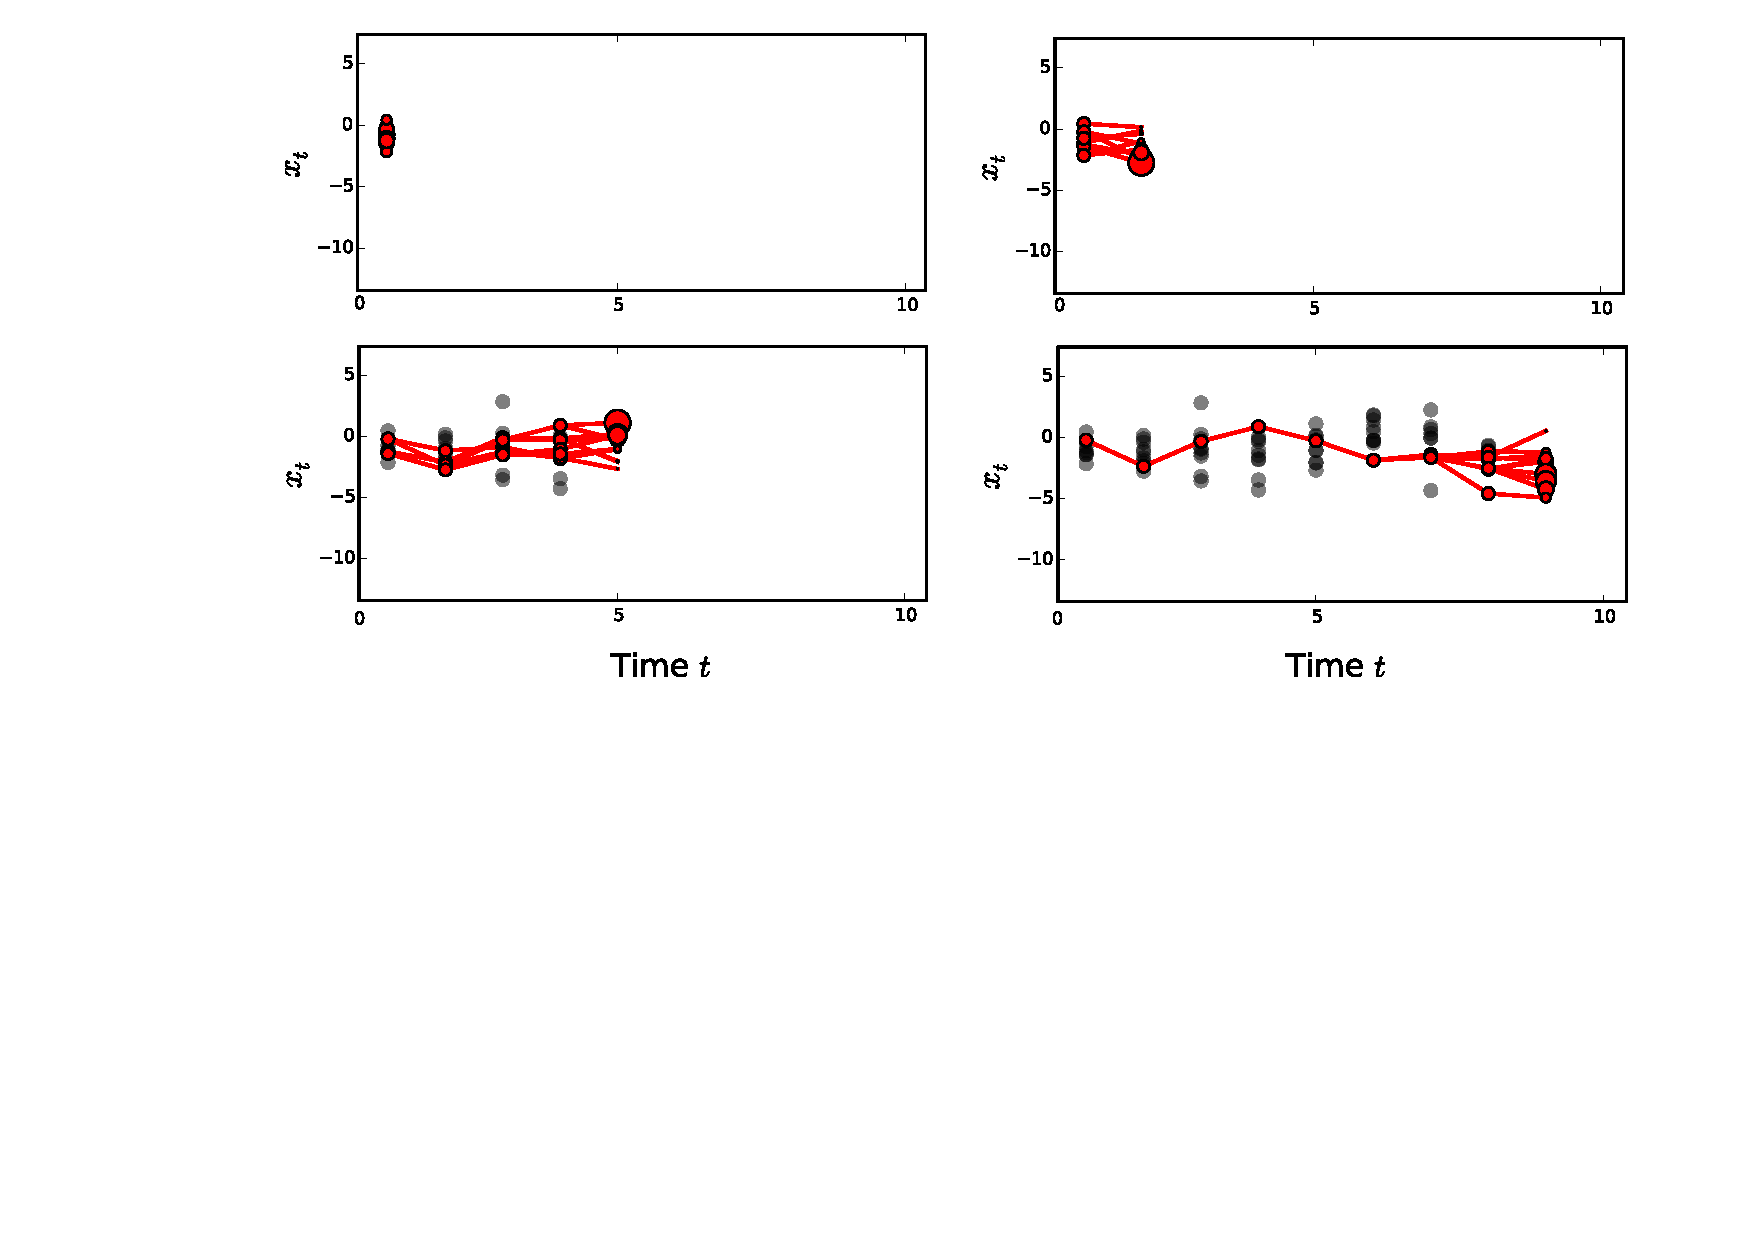
\includegraphics[width=\textwidth]{part/figures/smc_explan}
	\caption{Characterization of the SMC method for a state space model.  At the first time step (top left) 
		we perform importance sampling to approximate $p(x_1 | y_1)$ in the normal way, giving a particle system, or population
		of weighted samples $\{x_1^i,w_1^i\}_{i=1}^N$.  Here each sample is shown by a red blob whose size reflects the weight
		of the particle.  The set of particles are then resampled to produce an unweighted set of particles approximating
		$p(x_1 | y_1)$.  For each of these samples, importance sampling is then used again to produce samples for $x_2$
		by sampling from $q_2 (x_2 | x_1)$ and applying a new importance weight (top right).  Note that, unlike for SIS,
		the importance weights are not propagated from one time step to the next.
		We now again have a weight particle set $\{x_{1:2}^i,w_2^i\}_{i=1}^N$, for which we again perform a resampling
		step to produce an unweighted set of particles.  The process continues in the same way, eventually returning the
		final set of samples $\{x_{1:T}^i,\nw_T^i\}_{i=1}^N$, where we have self-normalized the final weights of each trajectory
		(note that each $\nw_T^i$ applies to the full trajectory $x_{1:T}^i$).  
		Over time, many of the generated samples are
		discarded by the system (shown in gray) during the resampling step.  A consequence of this, which can be seen
		in the bottom right, is that
		many time steps, then our particle set become \emph{degenerate}.  Here we have multiple distinct samples for $x_9$, but
		all our samples share the same \emph{ancestors} for $t=1:6$, i.e. each $x_t^i$ in our final sample set is
		the same for $t\le6$.  We will return to discuss this further in Section~\ref{sec:part:pmcmc:path-deg}.
		\label{fig:part:smc_explan}}
\end{figure}

To see the intuition of why resampling provides the desired resource reallocation, consider what happens 
to the relative weights of different particles in a population if they are propagated through the SIS algorithm at the
same time.  It is easy to see that these weights will quickly diverge, typically exponentially quickly
 (see Section~\ref{sec:inf:foundation:curse}), and our effective sample size 
(see Section~\ref{sec:inf:foundation:ess}) will rapidly diminish.  It is now rather pointless to continue to
propagate the samples with negligible weight through the system as the chance these will have a significant
weight by the end is very low.  We therefore desire a principled way of ``killing off'' these
low weight particles and replacing them with higher weight ones.  As we showed in Section~\ref{sec:inf:foundation:resampling},
resampling gives us a method for generating unweighted samples from a population of weighted samples.
Though resampling itself only duplicates existing particles, rather
than producing new ones, if the duplicate samples are extended independently at the next iteration, this
produces distinct samples (albeit heavily correlated ones).  In other words if we have two samples
$x_{1:t}^1$ and $x_{1:t}^2$ such that $w_t^2/w_t^1 \approx 0$ then it is more beneficial for us to generate both
samples at the next stage using $x_{t+1}^i \sim p(x_{t+1} | x_{1:t}^1, y_{1:t})$ for $i=1,2$, than to use
$x_{1:t}^2$ to sample $x_{t+1}^2$.  This will not improve our representation of $x_{1:t}$, but it will, in
general, give a better representation of the marginal distribution of $x_{t+1}$ and thus the joint distribution
$x_{1:t+1}$.   
%Note that any of the resampling schemes introduced in Section~\ref{sec:inf:foundation:resampling}
%will give rise to valid SMC schemes and so one should, from a practical perspective, generally
%use systematic resampling.

To introduce the \smc method more formally, we consider approximating a sequence of target distributions
in same way as for SIS: in our NMSSM
 case $p(x_{1:t}|y_{1:t}) = p(y_{1:t})^{-1} p(x_{1:t},y_{1:t}), ~t=1,\ldots,T$. 
At each time step $t$ we 
%assume we have access to 
generate a particle system
$\{x_{1:t}^i,w_{t}^i\}_{i=1}^N$ which provides a weighted approximation  to $p(x_{1:t}|y_{1:t})$. Given such a 
weighted particle system, we convert this to an unweighted particle system by resampling as explained
in Section~\ref{sec:inf:foundation:resampling}.  Any of the introduced resampling schemes can be 
used~\citep[Section 4.1]{andrieu2010particle}
and so in general one should use systematic resampling.
When we later introduce PMCMC methods, it will
be useful to think about resampling in terms of propagating particles each particle by drawing an 
ancestor variable $a_{t-1}^i$ (as per~\eqref{eq:inf:resampling}) and then using this to propose the new
variable for that particle, i.e. $x_t^i \sim q_t(x_t | x_{1:t-1}^{a_{t-1}^i})$.  The particle system is then
re-weighted as
\begin{align}
\label{eq:part:smcweights}
w_t^i = \frac{g_t(y_t|x_{1:t}^i) f_t(x_t^i | x_{1:t-1}^{a_{t-1}^i})}{q_t(x_t^i|x_{1:t-1}^{a_{t-1}^i})},
\end{align}
where $x_{1:t}^i = (x_{1:t-1}^{a_{t-1}^i},x_t^i)$.   Note that after resampling,
all the particles have the same weight and therefore, unlike for SIS, the weights at the previous step
do not feature in the weights at the current time step.
This results in a new particle system $\{x_{1:t}^i,w_t^i\}_{i=1}^N$ that approximates $p(x_{1:t}|y_{1:t})$
and the algorithm continues in a self-similar manner up to time $T$.
The overall process is detailed in Algorithm~\ref{alg:part:smc}.  Once run, we can use our final, self-normalized,
particle set $\{x_{1:T}^i,\nw_T^i\}_{i=1}^N$ as a Monte Carlo estimator in the same manner as self-normalized
importance sampling:
\begin{align}
\label{eq:part:smc-est}
\E_{\pi (x_{1:T})} \left[f(x_{1:T})\right] \approx \frac{1}{N} \sum_{i=1}^{N} \nw_T^i f(x_{1:T}^i).
\end{align}

\begin{algorithm}[tb]
	\caption{Sequential Monte Carlo \hfill {\small (all for $i=1,\ldots,N$)}}
	\label{alg:part:smc}
	\begin{spacing}{1.2}
		\begin{algorithmic}[1]
			\renewcommand{\algorithmicrequire}{\textbf{Inputs:}}
			\renewcommand{\algorithmicensure}{\textbf{Outputs:}}				 
			\Require  data $y_{1:T}$, number of particles $N$, proposals $q_t$
			\State $x_1^i \sim q_1(x_1)$
			\State $w_1^i = \frac{g_1(y_1|x_1^i) \mu(x_1^i)}{q_1(x_1^i)}$
			\For{$t = 2$ {\bfseries to} $T$}
			\State $a_{t-1}^i \sim \Discrete\left(\left\{\nw_{t-1}^{\ell}\right\}_{\ell=1}^N\right)$% \tom{We can maybe more general that categorical here?}
			\State $x_t^i \sim q_t(x_t | x_{1:t-1}^{a_{t-1}^i})$ 
			\State Set $x_{1:t}^i = (x_{1:t-1}^{a_{t-1}^i},x_t^i)$
			\State $w_t^i = \frac{g_t(y_t|x_{1:t}^i) f_t(x_t^i | x_{1:t-1}^{a_{t-1}^i})}{q_t(x_t^i|x_{1:t-1}^{a_{t-1}^i})}$
			\EndFor
		\end{algorithmic}
	\end{spacing}
\end{algorithm}

Many intuitions from importance sampling transfer over to SMC.  For example, we can construct our posterior
estimate and calculate expectations in the same way, while we can also use the effective sample size as
a metric of performance (remembering to coalesce identical samples). 
One of the most importance features that translates is that SMC produces the
unbiased estimate for the marginal likelihood $p(y_{1:T})$
\begin{align}
\label{eq:part:ML}
\hat Z = \prod_{t=1}^T \frac{1}{N} \sum_{i=1}^N w_{t}^{i}.
\end{align}
as first shown by~\cite{del2004feynman}.  Although this original
proof requires advanced techniques we will not touch on here, we will later show that this results can also be shown
as a consequence of the proof of correctness for the particle independent Metropolis-Hastings method
given in Section~\ref{sec:part:pmcmc:pimh}.  Note that although the marginal likelihood estimate is
unbiased, the estimator for an general expectation given by~\eqref{eq:part:smc-est} is biased in the same
way as the self-normalized importance sampling estimator given in~\eqref{eq:inf:snis} is.  Nonetheless, producing unbiased
estimates of the marginal likelihood has numerous significant advantages.  

Firstly, it means that one can combine
results from difference SMC runs and still have a consistent estimator for the target and a both unbiased and
consistent estimate for the marginal likelihood.
The is particularly important because the number of particles $N$, is typically restricted by the availability of memory
and we often want to run more than one \emph{SMC sweep} (i.e. single run of SMC).
To combine our estimates, one simply weights each sample by the marginal likelihood of its sweep times
its local, self-normalized, weight $\nw_T^i$, giving the estimator
\begin{align}
\label{eq:part:ind-smc}
\E_{\pi (x_{1:T})} \left[f(x_{1:T})\right] \approx \frac{1}{RN} \sum_{r=1}^{R}\sum_{i=1}^{N} \hat{Z}[r] \nw_T^i[r] f(x_{1:T}^i[r])
\end{align}
where the notation $[r]$ is used to indicates samples from sweep $r$.
 The ability to do this is known as \emph{proper weighting}~\citep{andersson2015nested} and we can justify it by
thinking in terms of using a proposal that first samples a full particle set, giving importance weight $\hat Z$, and then sampling a particle
from this set, giving importance weight $\nw_T^i$.  The product of these separate weights thus gives the weight of
each sample.  

Secondly, the unbiased marginal likelihood estimate means that we can \emph{nest} SMC within other 
methods as a unbiased estimate of the likelihood.
Methods that make use of such unbiased likelihood estimates are known as pseudo-marginal
methods~\citep{andrieu2009pseudo} and will be discussed in Chapter~\ref{chp:nest}.
Some PMCMC methods we introduce in Section~\ref{sec:part:pmcmc} (namely PIMH and PMMH) 
can also be interpreted as pseudo-marginal methods.
%
%The sequential nature of SMC and the resampling step are crucial in making SMC scalable to large $T$.
%The former makes it easier to design efficient proposal distributions as each step need only target 
%the next set of variables $x_t \in \mathcal{X}_t$. 
%The resampling step then allows the algorithm to focus on promising particles in light of new 
%observations, avoiding the exponential divergence between the weights of different samples that 
%occurs for importance sampling as $T$ increases.
%This can be demonstrated both empirically and theoretically \citep[Chapter 9]{del2004feynman}.

\subsection{Sequential Monte Carlo for an Arbitrary Series of Targets}
\label{sec:part:smc:arb}

In its most general form, we can use SMC to target an arbitrary
series of unnormalized target distributions $\left\{\gamma_t (x_{1:t})\right\}_{t=1:T}, \; 
\gamma_t (x_{1:t}) = Z_t \pi_t (x_{1:t})$, each defined on a space
$\mathbb{X}_t$ with strictly increasing dimension\footnote{This restriction
	can be relaxed by using the SMC samplers approach of \citet{del2006sequential}.}
$\mathrm{dim}(\mathbb{X}_{t-1})<\mathrm{dim}(\mathbb{X}_{t})$.
Here $Z_t := \int \gamma_t(x_{1:t}) dx_{1:t}$ is the normalization constant and $\pi_t (x_{1:t})$
the corresponding normalized target.  
The only difference that needs to be made from the NMSSM case is in how the weights
are calculated, with them now given by
\begin{subequations}
\label{eq:part:smc-arb-weights}
\begin{align}
w_1^k &= \frac{\gamma_1(x_1^k)}{q_1(x_1^k)} \\
w_t^k &= \frac{\gamma_t({x}_{1:t}^k)}{\gamma_{t - 1}({x}_{1:t - 1}^{a_{t - 1}^k}) q_t(x_t^i|x_{1:t-1}^{a_{t-1}^i})}.
\end{align}
\end{subequations}
It can be easily seen that the NMSSM weights are a particular case of this, by
plugging in $\gamma_t(x_{1:t}) = p(x_{1:t},y_{1:t})$ into the above expression.  

For inference, then our posterior is the
last target, $\pi_T (x_{1:T})$, with corresponding marginal likelihood $Z_T$.  Using this
more general SMC formulation, we thus see that any series of targets will lead
to a valid inference provided that the final target is the desired posterior and that none
of our intermediate targets place zero probability mass on events that have non-zero
probability mass under the corresponding marginals of the final target 
\begin{align}
\label{eq:part:opt-target}
\tilde{\pi}_t (x_{1:t}) = \int \pi_T (x_{1:T}) dx_{t+1:T}
\end{align}
$\ne \pi_t (x_{1:t})$ in general.  In fact, the series of targets given
for the NMSSM case are actually suboptimal and used because of the fact that
$p(x_{1:t},y_{1:t})$ can, in general, be calculated exactly.  It is a well known result
(see, for example, the appendices of~\cite{le2017auto}) that the optimal series
of proposals (complications with computability and proposals aside) is actually 
the marginals $\tilde{\pi}_t (x_{1:t})=p(x_{1:t} | y_{1:T})$ for
the NMSSM case.  To see this, note that at the $t^{\mathrm{th}}$ step, we are generating 
the samples for $x_{t}$ and so if each of targets is the marginal of the final distribution
$p(x_{1:t} | y_{1:T})$, then the marginal probability of the already sampled variables does not change from
one step to the next.  Conversely, $\pi_t (x_{1:t}) \neq \int \pi_{t+1} (x_{1:t+1}) dx_{t+1}$
in general and so if a different series of targets are used,
e.g. $p(x_{1:t}|y_{1:t})$, then the marginal probability of the already sampled
variables changes from one iteration to the next, reducing the efficient of the inference.
To give an example of this, consider
the case where $x_{1}$ include global parameters that effect each emission
distribution, for example it could contain the variance for Gaussian
likelihood terms.  In our NMSSM case we can never regenerate samples for $x_1$ after
the first step and so it is clearly better at the first step to target $p(x_1 | y_{1:T})$ than $p(x_1|y_1)$,
i.e. to condition on all the data rather than the first datapoint. Unfortunately, calculating
$p(x_1 | y_{1:T})$ itself generally requires a marginalization that is as difficult, or potentially
even more difficult, than the inference itself.  Hence the series of targets we introduced in
the NMSSM formulation are those that are usually used in practice.  However, we note that there are some
innovative methods for partially alleviating this problem, such as block sampling~\citep{doucet2006efficient} methods,
which use a combination of lookahead and \emph{auxiliary weighting} schemes~\citep{cappe2007overview}.
Specifically, they resample using adjusted weights that convey how good the sample is likely
to be a few time steps further down the line.  The bias this would induce is corrected for
by assigning non-even weights to the resampled particles.

Another upshot of the ability to use an arbitrary series of targets is that we can use SMC in scenarios that do not
permit a conventional breakdown of the target distribution, but where we 
can provide guiding distributions to that which we care about.  One possible case is when our prior distribution
is a generative model that can be evaluated on the target dataset at point in generative process.
For example, in~\cite{janz2016probstruct}, we considered the example of doing inference
on the structure of a GP kernel.  Here we can define a generative model that produces
increasingly complex kernels, such that all the intermediary kernels in this generation process are themselves
valid kernels that can thus be evaluated.  Here we can think of expanding our kernel at each time step of 
the SMC inference and our targets as being the posterior on kernel structure for the GP, subject to increasingly
lax restrictions on the kernel complexity.\footnote{Technically in this work actually uses population
	Monte Carlo~\cite{cappe2004population} which is based on using a series of static targets.  The
	intuition, however, predominantly transfers and SMC could have been used instead.}  
Another example is provided by~\cite{lakshminarayanan2013top},
who use SMC for Bayesian learning of decision trees.  Here they use the self-similarity of trees, starting
with a basic stump and then adding a new split at each time step.
For both these problems, SMC has been used
to exploit the fact that the overall problem can be broken down into a series of increasingly difficult
problems, namely those with an increasingly large prior, to guide towards good solutions for the final problem.

\subsection{Practical Considerations}
\label{sec:part:smc:prat}

\subsubsection{Use as Many Particles as Possible}
\label{sec:part:smc:prat:part}

The most important practical consideration for SMC is to
\emph{use as many particles as possible}.  Although, as we showed in~\ref{sec:part:smc:nmssm},
one can run multiple, say $R$, SMC sweeps with $N$ particles each and then combine them using their marginal likelihood estimates, this
is almost exclusively a higher variance (and more skew) estimator than carrying out a single SMC sweep
with $RN$ particles, often many orders of magnitude so.  It is easy to see why a single sweep is preferable
from the point of view of the effect of the different marginal likelihood estimates on the effective sample size.
The reason the number of particles can be so critical is that if it is too small, the variance of the marginal likelihood
estimate explodes, the effective sample size plummets, and one sweep ends up dominating the estimate.  Though the marginal 
likelihood estimate is unbiased, it has a massive positive skew when insufficient particles as used, such that the 
probability that a
sweep gives a marginal likelihood estimate larger than the true marginal likelihood estimate can be arbitrarily small;
after all, the limit $N=1$ corresponds to importance sampling.  As such, if we use insufficient particles and just
repeatedly run SMC sweeps, we may have to wait arbitrarily long before getting any useful samples.  One way 
to try an combat this, presuming it is not possible to increase $N$, is to group the SMC sweeps into a number
of islands and then combined estimates in the normal way within the islands, but combined the islands in
an unweighted fashion (see for example~\cite{lakshminarayanan2013top}).  Though often practically useful, this
is clearly only trading variance for bias and thus is more of a means of mitigating rather than solving the problem.
A more principled means of overcoming this issue is presented by PMCMC methods as discussed in Section~\ref{sec:part:pmcmc}.

\subsubsection{Adaptive Resampling}
\label{sec:part:smc:prat:ad-re}

Another important practical consideration is that it is not always beneficial to resample.  Resampling
obviously throws away information (by reducing the number of distinct particles)
and therefore should not be done spuriously.  As the reason for doing
resampling is to kill off particles with negligible weight, it is generally preferable to avoid the resampling step
when most particles have significant weight.  This lead to the development of so-called \emph{adaptive resampling}
schemes that only perform the resampling step if some criterion is met~\citep{liu1995blind,del2012adaptive}, e.g. 
only resampling when the effective sample size falls below a certain threshold,
for which $N/2$ is a common choice~\cite{doucet2009tutorial}.
When the resampling is omitted, the particles remain unweighted, with their weights at the next iteration updated
using~\eqref{eq:part:sis-weights}, as per SIS, except that the self normalized weights $\bar{w}_t^i$ should be used so that the
marginal likelihood estimate can be carried out in the same manner.
That this still informally forms a valid SMC algorithm for posterior inference can be seen by thinking of these as being sequential importance
sampling steps, noting the equivalence to standard importance sampling, and then viewing the process as simply
skipping some of the intermediate targets, remembering that it is only the final target that we care about.
However, adaptive resampling does cause some complications from a theoretical perspective~\citep{del2012adaptive}.

\subsubsection{Proposals}
\label{sec:part:smc:prat:opt}

The practical performance of SMC can be critically dependent on the choice of proposal and
so we finish our introduction by considering what constitutes a good proposal, first
considering the question of what the theoretically optimal proposal is. Unfortunately it is not generally
possible to establish the optimal proposal for the variance of the final estimate in the finite $N$ case, but we can
calculate the so-called \emph{one-step optimal proposal} by minimizing the variance of the individual weights (and
by proxy the marginal likelihood estimate) at the next iteration.  The one-step optimal proposal is given by
\begin{align}
\label{eq:part:opt-prop}
q_t^*(x_t | x_{1:t-1}) \propto \frac{\gamma_t({x}_{1:t})}{\gamma_{t - 1}({x}_{1:t - 1})} 
\end{align}
$= f_t(x_t | x_{1:t-1}) g_t(y_t | x_{1:t})$ for the NMSSM formulation.  To see why this is optimal we note that
by substituting~\eqref{eq:part:opt-prop} into~\eqref{eq:part:smc-arb-weights} (noting that the proposal needs
to be correctly normalized) then the weights are simply the normalization constant for~\eqref{eq:part:opt-prop}, namely
\begin{align}
w_t(x_{1:t}) &= \int \frac{\gamma_t({x}_{1:t})}{\gamma_{t - 1}({x}_{1:t - 1})} dx_t = 
\frac{\int\gamma_t({x}_{1:t}) dx_t}{\gamma_{t - 1}({x}_{1:t - 1})} 
\end{align}
$=p(y_t | x_{1:t-1})$ for the NMSSM formulation.  Consequently, the weights in the this case are no longer
functions of the sampled value and so the marginal likelihood and effective sample size are deterministic
functions of the particle system before proposing the $x_{t}$, namely of $\{x_{1:t-1}^i,a_{t-1}^i\}_{i=1}^N$.
This also means that we can switch the order of sampling from the proposal and doing the resampling when
using $q_t^*(x_t | x_{1:t-1})$, which is preferable as it increases the diversity in the final sample set.
Note that the weights are not all the same when using the one-step optimal proposal, because
the marginal probability of the particles will change when we incorporate the new observation (or equivalently
move to the new target).  However, given the expected value of each weight is fixed, i.e. $\E [w_t(x_{1:t}) | x_{1:t-1}]=
\frac{\int  \gamma_t({x}_{1:t}) dx_t}{\gamma_{t - 1}({x}_{1:t - 1})} $ regardless of the proposal
used, using any proposal other than the optimal one-step proposal only increases the variance of the estimate
at the next step.  In particular, it is generally
not beneficial to use proposals that include some form of lookahead (e.g. approximating $p(x_{t} |x_{1:t-1},y_{1:T})$
instead of $p(x_{t} |x_{1:t-1},y_{1:t})$), because the resampling step will correct back to the current target and
most likely kill off the ``good'' samples we generated, simply giving us fewer distinct samples than if we had
used the one-step optimal proposal instead.\footnote{Note that lookahead in the proposal is distinct from
	lookahead using auxiliary weights, thus things like block sampling are still useful.}
In both the case where the optimal series of targets~\eqref{eq:part:opt-target} is used and in the large $N$ case, then
the one-step optimal proposal is optimal more generally for the whole SMC sweep for a given series of targets.  However, because it is
not usually possible to analytically calculate the required normalization for $q_t^*(x_t | x_{1:t-1})$, it is
not generally tractable.  Nonetheless, it provides a good guide for designing, or adapting for, effective proposal
distributions.

Another proposal of note, at least for the state space model case, is the so-called bootstrap proposal which
corresponds to sampling from the transition distribution $f_t(x_t | x_{1:t-1})$.  The significance of this proposal
is that it means that the weight calculation given in~\eqref{eq:part:smcweights} cancel to
\begin{align}
\label{eq:part:bootstrap-weights}
w_t^i = g_t (y_t | x_{1:t}^i).
\end{align}
Consequently, if we use the bootstrap proposal we do not need to be able to evaluate the transition distribution
at a particular point, only sample from it.  Obviously this can be helpful for computational reasons (though
it is rare that the effect of this outweighs using a better proposal if one is known), but it is also important
because it can be the case that one only has access to a sampler for the transition and not the ability to evaluate
the transition probability at an arbitrary point.
In the absence of other information, the bootstrap can also be a reasonable choice of proposal in its own right as
it is almost always more diffuse than the one step posterior.  Its efficiency will in general depend on how relatively
peaked the emission distribution is and the dimensionality of $x_t$ -- after all, each step in SMC is in
isolation importance sampling.  One can usually beneficially use the next observation $y_t$ to help guide the
the proposal, but doing this in a general purpose manner can be challenging~\citep{gu2015neural}.
% !TEX root = ../main.tex

\section{Particle Markov Chain Monte Carlo Methods}
\label{sec:part:pmcmc}

Particle Markov chain Monte Carlo (\pmcmc) methods, introduced by \citet{andrieuDH2010}, make use of 
sequential Monte Carlo (\smc) algorithms \citep{gordon1993novel,doucet2001sequential} to construct 
efficient proposals for an \mcmc sampler. This allows it to both utilize the ability of SMC to
exploit the structure of the target problem and the hill climbing behavior of MCMC methods.
The critical difference from running independent SMC sweeps is that information can be transferred
from sweep to the next. 
%The core reason for wanting to do this is that
%one is typically memory restricted in the number of particles that can be run $N$.  Though as we explained
%before, we can run multiple sweeps and combine these using the marginal likelihood estimates, if $N$ is
%not large enough, this typically results it widely varying estimates.  Although these estimates are unbiased,
%they are typically extremely skew, often following a roughly Gaussian distribution in their \emph{log} marginal
%likelihood CITE SOMETHING.  As such, it usually happens if $N$ is not large enough that one sweep dominates the others because
%its marginal likelihood is many orders of magnitude larger than the others and our estimate is
%effectively just the particle sweep with the highest marginal likelihood.  We therefore desire a more principled
%means of transferring the information of one iteration to the next which we can do by constructing an appropriate MCMC
%sampler.  We can then combine the advantages of SMC in its exploitation of the structure of the target with
%the local updating advantages of MCMC methods.  
Naturally this will come with the drawbacks of MCMC samplers
discussed in Section~\ref{sec:inf:foundation:mcmc}, in particular the loss of unbiasedness or marginal likelihood estimates.
However, the advantages will generally outweigh these drawbacks.  PMCMC methods will also allow us to explicitly
treat global parameters of our system differently to the latent states in a manner that can substantially improve
the performance of the model.
Though PMCMC can be applied to models with arbitrary series of targets in the same manner as SMC, we will stick
to the NMSSM case in this section for notational simplicity.

\subsection{Particle Independent Metropolis Hastings}
\label{sec:part:pmcmc:pimh}

Particle independent Metropolis Hastings (PIMH) is the simplest PMCMC algorithm.  Although in isolation it is
not especially useful (as it strictly worse than running independent SMC sweeps and combining 
them),\footnote{There is, though, utility in doing this when also including MCMC steps on global parameters, see~\cite{andrieu2010particle}.}
 it is an
important theoretical stepping stone to more advanced approaches.  The idea from a practical perspective 
is very simple: use an SMC sweep as an independent proposal for an MCMC algorithm targeting $\pi(x_{1:T}) = p(x_{1:T}|y_{1:T})$.
From a theoretical perspective, the approach is rather more profound as it can be viewed as a sampler on 
an \emph{extended space} whose marginal on the returned particles is the target.  
%We will then be able to use
%this to construct more powerful samplers.

\begin{algorithm}[tb]
	\caption{Particle Independent Metropolis Hastings}
	\label{alg:part:pimh}
	\begin{spacing}{1.2}
		\begin{algorithmic}[1]
			\renewcommand{\algorithmicrequire}{\textbf{Inputs:}}
			\renewcommand{\algorithmicensure}{\textbf{Outputs:}}				 
			\Require SMC sampler, number of MCMC iterations R
			\Ensure MCMC samples $\{\hat{x}_{1:T}^r\}_{r=1}^R$
			\State Run SMC giving particle set $X_{1:T}^0 = \{x_{1:T}^{i,0},w_T^{i,0}\}_{i=1}^N$ and marginal likelihood $\hat{Z}^0$
			\State Sample a single particle from set $\hat{x}_{1:T}^0 \sim X_{1:T}^0$ with probability proportional to weight
			\For{$r=2:R$}
			\State Run SMC giving candidate $\tilde{X}_{1:T}^r = \{x_{1:T}^{i,r},w_T^{i,r}\}_{i=1}^N$
				 and $\tilde{Z}^r$
			\If{$u\le \min \left(1,\frac{\tilde{Z}^r}{\hat{Z}^{r-1}}\right)$ where $u\sim \textsc{Uniform}(0,1)$}
			\State $\hat{x}_{1:T}^r \sim \tilde{X}_{1:T}^r, \quad \hat{Z}^{r} \leftarrow \tilde{Z}^r$
			\Else
			\State $\hat{x}_{1:T}^r \leftarrow \hat{x}_{1:T}^{r-1}, \quad \hat{Z}^{r} \leftarrow \hat{Z}^{r-1}$
			\EndIf
			\EndFor
		\end{algorithmic}
	\end{spacing}
\end{algorithm}

The PIMH algorithm is given in Algorithm~\ref{alg:part:pimh}.  We see that PIMH is an MCMC
algorithm where our proposal involves running an independent SMC
sweep and then sampling one of the particles from this particle set in proportion to
the weight of the particle.  This sample is then accepted or rejected using a MH accept-reject
step that  uses the marginal likelihoods of the sweep.  Because our proposal
is independent of our current point, this is strictly worse than just running independent SMC sweeps
(which can also be thought of as applying waste recycling to PIMH ~\citep{frenkel2006waste}).  
It might seem wasteful to only use
one particle from each sweep, but we will be able to Rao-Blackwellize this step and actually
return all the particles at each step as we explain in Section INSERT. 

%Imagine that we were able to exactly calculate the posterior probability of the of samples
%generated by an SMC sweep up to a normalization constant $\gamma(X_{1:T} |y_{1:T})$.  It would
%now be straightforward to construct a valid sampler on this distribution by constructing an independent
%MH proposal and accept/reject the particle sets in the standard way.
The key component of proving the correctness of the PIMH algorithm is in showing that it is a valid
MH sampler on an extended target whose marginal is the distribution of interest.
%The two key components of proving
%the correctness of the PIMH algorithm are in showing that running and SMC sweep then sampling
%one of the samples produced an extended target distribution whose normalized marginal distribution is
%the posterior of interest $\pi(x_{1:T}|y_{1:T})$ and that our MH algorithm remains valid when
%provided with an \emph{unbiased estimate} of the target distribution rather than an exact calculation.
Let $\xib \eqdef \{x_{t}^i\}_{\substack{i=1:N\\t=1:T}} \bigcup \{a_{t}^i\}_{\substack{i=1:N\\t=1:T-1}}$
denote all generated particles and ancestor variables of a \smc sampler.  The density of the distribution induced
by running a SMC sweep is now given by
\begin{align}
\label{eq:part:smc:proposal}
q_{\text{SMC}}(\xib) &= \prod_{i=1}^N q_1(x_{1}^i) \cdot \prod_{t=2}^T \prod_{i=1}^N \left[ 
\nw_{t-1}^{a_{t-1}^i}
%\frac{w_{t-1}^{a_{t-1}^i}}{\sum_\ell w_{t-1}^{\ell}}
q_t(x_{t}^i|x_{1:t-1}^{a_{t-1}^i}) \right]
\end{align}
and the distribution induced by running an SMC sweep and then sampling particle $b$ from the
sample set is 
\begin{align}
q_{\text{PIMH}}(\xib,b) = \bar{w}_T^b q_{\text{SMC}}(\xib) \quad \text{where} \quad \bar{w}_t^i = \frac{{w}_t^i}{\sum_{\ell=1}^{N}w_t^{\ell}}.
\end{align}
Let $\xb^i = x_{1:T,m}^i$ denote one of the final particles and let the trajectory associated
with the particle we sample be $\{\xb^{b},\bb\}$, with $\bb = (\beta_{1,},\ldots,\beta_{T})$,
$\beta_{T} = b$ and $\beta_{t} = a_{t}^{\beta_{t+1}}$. The proof for the validity of the PIMH
algorithm is now demonstrated by showing that it a valid MH sampler for an \emph{extended target distribution}
whose marginal distribution on $\xb^b$ is the distribution of interest $\pi(\xb^b)$.  To construct our
extended target distribution, we consider the following hypothetical sampling process
\begin{enumerate}
	\item Sample a particle exactly from the target $\xb^b \sim \pi(\xb^b)$,
	\item Sample a path for the particle uniformly at random path by independently sampling each $\beta_t \sim \textsc{UniformDiscrete}(1,N)$,
	\item Sample all of the other particles and trajectories conditioned on $\{\xb^{b},\bb\}$ using \begin{align}
	\label{eq:part:csmc}
	q_{\text{CSMC}}\left(\xib \backslash \{\xb', \bb\} \mid \xb', \bb \right) = 
	\prod_{\substack{i=1\\i\neq b_{1}}}^N  q_1(x_{1}^i) \cdot \prod_{t=2}^T \prod_{\substack{i=1\\i\neq b_{t}}}^N \left[
	\nw_{t-1}^{a_{t-1}^i}q_t(x_{t}^i|x_{1:t-1}^{a_{t-1}^i})\right].
	\end{align}
\end{enumerate}
Together these steps induce the distribution
\begin{align}
\label{eq:part:pimh-target}
\tilde{\pi}(\xi,b) = \frac{\pi(\xb^{b})}{N^T} \prod_{i=1, i\neq\beta_1}^N q_1(x_{1}^i) \cdot \prod_{t=2}^T \prod_{i=1, i\neq\beta_t}^N \left[ 
\nw_{t-1}^{a_{t-1}^i}
q_t(x_{t}^i|x_{1:t-1}^{a_{t-1}^i}) \right].
\end{align}
By construction, the marginal of this distribution is $\pi(\xb^{b})$.
Therefore, although it is not possible to actually
sample from $\tilde{\pi}(\xi,b)$ directly (we started the definition by sampling exactly
from the distribution of interest), if we can
construct a consistent MCMC estimator on~\ref{eq:part:pimh-target} then this by proxy
produces a consistent estimator for $\pi(\xb^{b})$.
We can now show that this is exactly what the
PIMH algorithm does by explicitly calculating the importance weight implied by
targeting $\tilde{\pi}(\xi,b)$ using the proposal $q_{\text{PIMH}}(\xib,b)$
\begin{align}
\frac{\tilde{\pi}(\xi,b)}{q_{\text{PIMH}}(\xib,b)} &= \frac{\pi(\xb^{b}) q_{\text{CSMC}}\left(\xib \backslash \{\xb', \bb\} \mid \xb', \bb \right)}
{N^T \bar{w}_T^b q_{\text{SMC}}(\xib)} \\
&= \frac{\pi(\xb^{b})}{N^T \bar{w}_T^b q_1(x_1^{\beta_1}) \prod_{t=2}^{T} \bar{w}_{t-1}^{\beta_{t-1}} q_t(x_t^{\beta_t} | x_{t-1}^{\beta_{t-1}})} \nonumber \\
&= \left(\frac{\gamma(\xb^{b})/Z}{
	q_1(x_1^{\beta_1}) \prod_{t=2}^{T} q_t(x_t^{\beta_t} | x_{t-1}^{\beta_{t-1}})}\right) \cdot
	\left( \frac{1}{N^T \bar{w}_T^b\prod_{t=2}^{T} \bar{w}_{t-1}^{\beta_{t-1}}} \right) \nonumber \\
&= \left(\frac{w_T^b}{Z}
	 \prod_{t=2}^{T} w_{t-1}^{\beta_{t-1}}\right)\cdot\left(
	\frac{1}{N^T \bar{w}_T^b \prod_{t=2}^{T} \bar{w}_{t-1}^{\beta_{t-1}}}\right) \nonumber \\
&= \left(\frac{w_T^b}{Z}
	\prod_{t=2}^{T} w_{t-1}^{\beta_{t-1}}\right)\cdot\left(
	\frac{\prod_{t=1}^T \frac{1}{N} \sum_{\ell=1}^N w_{t}^{\ell}}{w_T^b \prod_{t=2}^{T} w_{t-1}^{\beta_{t-1}}}\right) \nonumber \\
&= \frac{1}{Z} \prod_{t=1}^T \frac{1}{N} \sum_{\ell=1}^N w_{t}^{\ell}
= \frac{\hat{Z}}{Z}.
\end{align}
We thus have that $\hat{Z}$ is the importance weight for sampling the unnormalized
version of the target $\tilde{\gamma}(\xi,b) = Z \tilde{\pi}(\xi,b)$ and so using the
ratio of marginal likelihood estimates provides is exactly the acceptance ratio required for
the MH sampler.  We
have therefore proven that the PIMH algorithm induces a consistent Markov chain for
the target $\pi(x_{1:T})$.

Note that as an aside, this also shows the unbiasedness of the SMC marginal likelihood estimate
as we see that
\begin{align}
\E_{q_{\text{SMC}}(\xib)} \left[\hat{Z}\right] = \E_{q_{\text{PIMH}}(\xib,b)} 
\left[\hat{Z}\right]=\E_{\tilde{\pi}(\xi,b)} \left[Z\right]=Z.
\end{align}
However, SMC will not, in general, provide unbiased estimates for expectations of
functions, for the same reasons that self-normalized importance sampling gives biased
estimates of expectations (see Section~\ref{sec:inf:foundation:importance:self-norm}).

\subsection{Particle Gibbs}
\label{sec:part:pmcmc:pgibbs}

One particularly widely used \pmcmc algorithm is particle Gibbs (\pg). The \pg algorithm modifies the 
\smc step in the \pmcmc algorithm to sample the latent variables conditioned on an existing particle
 trajectory, resulting in what is called a conditional sequential Monte Carlo (\csmc) step. The \pg method
  was first introduced as an efficient Gibbs sampler for latent variable models with static parameters 
  \citep{andrieuDH2010}. Since then, the \pg algorithm and the extension by \citet{lindstenJS2014} have 
  found numerous applications in \eg Bayesian non-parametrics \citep{ValeraFSPC2015,tripuraneni2015}, 
  probabilistic programming \citep{wood2014new,vandemeent_aistats_2015} and graphical models 
  \citep{everitt2012,naessethLS2014,naessethLS2015nested}.  

The \pg algorithm targets the same extended target $\tilde{\pi}(\xib,b)$ as the PIMH algorithm defined
in~\ref{eq:part:pimh-target}, but rather than constructing a MH sampler with independent proposals for
this target, it constructs a Gibbs sampler.  This is done by iteratively 
running \emph{conditional} sequential Monte Carlo (\csmc) sweeps. As described in Algorithm~\ref{alg:csmc},
a \csmc sweep is similar to a standard, unconditional \smc sweep, except that it starts
with an existing \emph{conditional trajectory} $x_{1:T}'$, known as a \emph{retained particle} in the \pg
context, and runs the sweep conditioned on this conditional trajectory being present in the final sample
set.  One can think of this as running a SMC sweep conditioned on the predefined particle surviving each
of the resampling steps.  In other words, the other particles can sample the retained particle as an
ancestor but not vice versa, with the values and ancestral path of the retained particle prefixed. 
 In Algorithm~\ref{alg:csmc} we have
presumed  that this ancestral path is $\bb = (N,\dots,N)$ which is not always the case from a theoretical
perspective.  However, because the path is fixed up front, all possible paths are equivalent from the point
of view of running the sweep.  Therefore,
given we only actually care about the $\xb$ sampled by the algorithm and not the ancestral paths themselves,
we can just use a convenient fixed ancestral path for the retained particle in practice, as done in Algorithm~\ref{alg:csmc}.

\begin{algorithm}[tb]
	\caption{Conditional sequential Monte Carlo}
	\label{alg:csmc}
	\begin{spacing}{1.2}
		\begin{algorithmic}[1]
			\renewcommand{\algorithmicrequire}{\textbf{Inputs:}}
			\renewcommand{\algorithmicensure}{\textbf{Outputs:}}				 
			\Require data $y_{1:T}$, number of particles $N$, proposals $q_t$, conditional trajectory $x_{1:T}'$
			\State $x_1^i \sim q_1(x_1), ~i=1,\ldots,N-1$ and set $x_1^N = x_1'$
			\State $w_1^i = \frac{g_1(y_1|x_1^i) \mu(x_1^i)}{q_1(x_1^i)}, ~i=1,\ldots,N$
			\For{$t = 2$ {\bfseries to} $T$}
			\State $a_{t-1}^i \sim \Discrete\left(\left\{\nw_{t-1}^\ell\right\}_{\ell=1}^N\right), ~i=1,\ldots,N-1$
			\State $x_t^i \sim q_t(x_t | x_{1:t-1}^{a_{t-1}^i}), ~i=1,\ldots,N-1$
			\State Set $a_{t-1}^N = N$ and $x_t^N = x_t'$
			\State Set $x_{1:t}^i = (x_{1:t-1}^{a_{t-1}^i},x_t^i), ~i=1,\ldots,N$
			\State $w_t^i = \frac{g_t(y_t|x_{1:t}^i) f_t(x_t^i | x_{1:t-1}^{a_{t-1}^i})}{q_t(x_t^i|x_{1:t-1}^{a_{t-1}^i})}, ~i=1,\ldots,N$
			\EndFor
		\end{algorithmic}
	\end{spacing}
\end{algorithm}

Unlike \smc sweeps, \csmc sweeps can be linked together by conditioning each sweep using a \emph{retained particle}
sampled from the previous sweep with probability proportional to the final particle weights $\bar{w}^i_T$.
Therefore, once initialized, say using a standard \smc sweep, one can iterate between sampling a retained
particle in the same manner ancestor indices are sampled and running \csmc sweeps conditioned on this
retained particle.  Considerations about global parameters aside (see Section INSERT), this is know
as iterated \csmc and constitutes the \pg algorithm.  A characterization is provided in INSERT. 

\todo[inline]{Add PG characterization figure.}

The theoretical justification for the \pg algorithm can be shown in a similar manner as the PIMH algorithm.
The sampled index $b$ now corresponds the index of the retained particle and we can think of the
approach as alternating between Gibbs updates on $b$ and $\xib \backslash \{\xb,\bb\}$.    In other
words, we alternate between sampling $b \sim \tilde{\pi}(\cdot | \xib)$ and 
$\xib \backslash \{\xb,\bb\} \sim \tilde{\pi}(\cdot | \xb,\bb)$.  \todo[inline]{Continue here}


Though \pg allows for inference over both latent variables and static parameters, 
we will in this paper focus on sampling of the former.  

A drawback of PG is that it can be particularly adversely affected by \emph{path degeneracy} in the CSMC step.  Conditioning on an existing trajectory means that whenever resampling of the trajectories results in a common ancestor, this ancestor must correspond to this trajectory.  Consequently, the mixing of the Markov chain for the early steps in the state sequence can become very slow when the particle set typically coalesces to a single ancestor during the CSMC sweep.
We address this next with the iPMCMC algorithm.

\todo[inline]{Rao-Black}

%In the same way as above for the standard \smc algorithm we can define a joint probability distribution induced by running Algorithm~\ref{alg:csmc} %$q_{\text{CSMC}}(\xb^{1:N},\ab^{1:N}\backslash\{\xb^N,\bb^N\} | \xb^N,\bb^N)$, induced by running Algorithm~\ref{alg:csmc}, where $\xb^N, \bb^N$ is the retained (conditioning) particle. 
%\begin{align}
%&q_{\text{CSMC}}\left(\xb^{1:N},\ab^{1:N} \backslash \{\xb^N, \bb^N\} \mid \xb^N, \bb^N, k \right) = \nonumber \\
%&\prod_{\substack{i=1\\i\neq b_{1}}}^N \left[ q_1(x_{1}^i) \right] \prod_{t=2}^T \prod_{\substack{i=1\\i\neq b_{t}}}^N \left[\frac{W_{t-1}^{a_{t-1}^i}}{\sum_\ell W_{t-1}^\ell} q_t(x_{t}^i|x_{1:t-1}^{a_{t-1}^i})\right],
%\end{align}
%where $\xb^N, \bb^N$ is the retained (conditioning) particle.
%\brooks{doesn't make sense --- if the retained particle is $N$, why is it $\xb_m^k, \bb_m^k$ in the above equation? shouldn't $\xb_m^{1:N},\ab_m^{1:N} \backslash \{\xb_m^k, \bb_m^k\}$ actually be $\xb_m^{1:N-1},\ab_m^{1:N-1}$?}


%
%   Limitations
%
%\subsection{Parallelisation and Limitations}
%\label{sec:limitations}
%Our main goal is to increase the efficiency of particle \mcmc, particle Gibbs especially, by coupling independent \smc methods with \csmc algorithms, perhaps running on different workers or threads. The method we propose, interacting particle Markov chain Monte Carlo (\ipmc), makes efficient use of multi-core and distributed computing architectures to increase accuracy of the Monte Carlo sampler.

%The basic \pg typically suffers from the \emph{path degeneracy} effect of \smc samplers, \ie sample impoverishment due to frequent resampling, which leads to bad mixing of the Markov chain. Since we force one trajectory, the conditional part, to survive to the end it means that for early time steps we will almost always pick the corresponding sample from last iteration. To counteract this we might need a very high number of particles to get good mixing for all latent variables $x_{1:T}$, which can be infeasible due to e.g.~limited available memory. The \ipmc can alleviate this issue by a non-standard coupling of several conditional and unconditional (standard) \smc algorithms. The algorithm lets us, from time to time, completely switch out a \csmc particle system with a completely independent \smc one, resulting in improved mixing of the Markov chain.


% !TEX root = ../../main.tex

\begin{savequote}[8cm]
	An approximate answer to the right problem is worth a good deal more than 
	an exact answer to an approximate problem.
	\qauthor{--- John Tukey}
\end{savequote}


\section{Interacting Particle Markov Chain Monte Carlo}
\label{sec:part:ipmcmc}

In this section we introduce \emph{interacting particle Markov chain Monte Carlo} (\ipmcmc), a \pmcmc method based on an interacting pool of standard and conditional sequential Monte Carlo samplers. Like related methods, \ipmcmc is a Markov chain Monte Carlo sampler on an extended space. We present empirical results that show significant improvements in mixing rates relative to both non-interacting \pmcmc samplers, and a single \pmcmc sampler with an equivalent memory and computational budget. 
An additional advantage of the \ipmcmc method is that it is suitable for distributed and multi-core architectures.  

%!TEX root = ../../main.tex

In this section we introduce \emph{interacting particle Markov chain Monte Carlo} (\ipmcmc)~\citep{rainforth2016interacting}
a \pmcmc method based on an interacting pool of standard and conditional sequential Monte Carlo samplers. Like 
other PMCMC methods, \ipmcmc is a Markov chain Monte Carlo sampler on an extended space. In \ipmcmc we run a pool of 
\csmc and unconditional \smc algorithms as parallel processes that we refer to as nodes. After each run of this pool, 
we apply successive Gibbs updates to the indexes of the \csmc nodes, such that the indices of the \csmc nodes changes. 
Hence, the nodes from which retained particles are sampled can change from one MCMC iteration to the next, reducing
the sensitivity to path degeneracy relative to \pg 
by trading off exploration (\smc) and exploitation (\csmc) to achieve improved mixing of the Markov chains. Crucially, 
the pool provides numerous candidate indices at each Gibbs update, giving a significantly higher probability that an 
entirely new retained particle will be ``switched in'' than in non-interacting alternatives.

We prove that \ipmcmc is a partially collapsed Gibbs sampler on the extended space containing the particle sets for all nodes. 
In the special case where \ipmcmc uses only \emph{one} \csmc node, it can in fact be seen as a non-trivial and unstudied 
instance of the $\alpha$-\smc-based \citep{whiteley2016} \pmcmc method introduced by \citet{huggins2015}. 
However, with \ipmcmc we extend this further to allow for an arbitrary number of \csmc and standard \smc algorithms 
with interaction.

The interaction between nodes requires only minimal communication; each node must report an estimate of the marginal likelihood 
and receive a new role (\smc or \csmc) for the next sweep. This means that \ipmcmc is embarrassingly parallel 
and can be run in a distributed manner on multiple computers.  However, the advantages of \ipmcmc go far beyond
simple parallelization: our experimental evaluation shows that \ipmcmc outperforms both equivalent
non-interacting \pmcmc samplers as well as a single \pg sampler with the same number of particles run longer
to give a matching computational budget.
An implementation of iPMCMC is provided in the probabilistic programming system
\emph{Anglican}\footnote{\angurl} \citep{wood2014new} as we discuss in Chapter~\ref{chp:proginf}.  A general 
purpose toolbox for carrying out iPMCMC and other SMC / PMCMC inference in MATLAB is also provided by the custom
made \emph{probabilistic MATLAB} package.\footnote{\url{https://github.com/twgr/probabilistic_matlab}}
% !TEX root = ../../main.tex

% Here we describe the proposed method and its theoretical properties
\subsection{Method}
\label{sec:method}
%Our main goal with the interacting particle Markov chain Monte Carlo method is to increase the efficiency of particle \mcmc, particle Gibbs especially, by coupling independent \smc methods with \csmc algorithms, perhaps running on different nodes or threads. The method we propose, interacting particle Markov chain Monte Carlo (\ipmc), makes efficient use of multi-core and distributed computing architectures to increase accuracy of the Monte Carlo sampler.

The main goal of \ipmcmc is to increase the efficiency of \pmcmc, in particular \pg. 
As we explain in Section~\ref{sec:part:pmcmc:path-deg}, \pg is especially
susceptible to the \emph{path degeneracy} effect of \smc samplers because the early
time steps in the state-sequence can become stuck in the same position for long
periods if the ancestral paths in the \csmc sweeps typically coalesce to a single sample,
which is by construction guaranteed to be the retained particle.
%The basic \pg algorithm is especially susceptible to the \emph{path degeneracy} effect of \smc samplers, \ie sample impoverishment due to frequent resampling.  Whenever the ancestral lineage collapses at the early stages of the state sequence, the common ancestor is, by construction, guaranteed to be equal to the retained particle.  
This results in high correlation between the samples, and poor mixing of the Markov chain. %Since we force one trajectory, the conditional part, to survive to the end it means that for early time steps we will almost always pick the corresponding sample from last iteration. 
To counteract this we might need a very high number of particles to get good mixing for all latent variables $x_{1:T}$, which can be infeasible due to e.g.~limited available memory. \ipmc can alleviate this issue by, from time to time, switching out a \csmc particle system with a completely independent \smc one, resulting in improved mixing.

\ipmcmc, summarized in Algorithm~\ref{alg:ipmc}, consists of $M$ interacting separate \csmc and \smc algorithms, exchanging only very limited information at each iteration to draw new \mcmc samples. We will refer to these internal \csmc and \smc algorithms as nodes, and assign an index $m=1,\ldots,M$. 
At every iteration, we have $P$ nodes running local \csmc algorithms, with the remaining
$M-P$ nodes running independent \smc.
The \csmc nodes are given an identifier $c_j \in \{1,\ldots,M\}, ~j=1,\ldots,P$ with $c_j \neq c_k,~k \neq j$ and we write $c_{1:P} = \{c_1,\ldots,c_P\}$. Let $\xb_m^i = x_{1:T,m}^i$ be the internal particle trajectories of node $m$.

\begin{algorithm}[tb]
	\caption{\ipmcmc sampler}
	\label{alg:ipmc}
	\begin{spacing}{1.2}
	\begin{algorithmic}[1]
		\renewcommand{\algorithmicrequire}{\textbf{Inputs:}}
		\renewcommand{\algorithmicensure}{\textbf{Outputs:}}				 
		\Require number of nodes $M$, conditional nodes $P$ and \mcmc steps $R$, initial $\xb_{1:P}'[0]$
		\For{$r = 1$ {\bfseries to} $R$}
		\State Workers $1:M \backslash c_{1:P}$ run Algorithm~\ref{alg:part:smc} (\smc)
		\State Workers $c_{1:P}$ run Algorithm~\ref{alg:csmc} (\csmc), conditional on $\xb_{1:P}'[r-1]$ respectively.
		\For{$j = 1$ {\bfseries to} $P$}
		\State Select a new conditional node by simulating $c_j$ according to \eqref{eq:simConditional}. %with probability 
		\State Set new \mcmc sample $\xb_j'[r] = \xb_{c_j}^{b_j}$ by simulating $b_j$ according to~\eqref{eq:simTrajectory}
		\EndFor
		\EndFor
	\end{algorithmic}
\end{spacing}
\end{algorithm}

Suppose we have access to $P$ trajectories ${\xb_{1:P}'[0]=(\xb_1'[0],\ldots,\xb_P'[0])}$ corresponding to the initial retained particles, where the index $[\cdot]$ denotes \mcmc iteration. At each iteration $r$, the nodes $c_{1:P}$ run \csmc (Algorithm~\ref{alg:csmc}) with the previous \mcmc sample $\xb_j'[r-1]$ as the retained particle. The remaining $M-P$ nodes run standard (unconditional) \smc, \ie Algorithm~\ref{alg:part:smc}.  Each node $m$ returns an estimate of the marginal likelihood $\hat Z_{m} $ for the internal particle system
calculated as per~\eqref{eq:part:ML}.  Note that whereas for the \smc sweeps this is an unbiased estimate of the 
marginal likelihood, this a biased estimator for the \csmc sweeps that is being specifically defined for our purposes.
%\begin{align}
%\label{eq:ML}
%\hat Z_{m} = \prod_{t=1}^T \frac{1}{N} \sum_{i=1}^N w_{t,m}^{i}.
%\end{align}
%along with a single trajectory $\xb_{m}^{s_m}$ sampled according to 
%\begin{align}
%\label{eq:simTrajectory}
%\Prb(s_m = i) &= \nw_{T,m}^i
%\end{align}
%where $s_m$ is the local index of the sampled particle.  

The new conditional nodes are then set using a single loop $j=1:P$ of Gibbs updates, sampling new indices $c_j$ where
\begin{align}
\label{eq:simConditional}
&\Prb(c_j = m|c_{1:P\backslash j}) = \hat\nz_{m}^j \\
\label{eq:zeta_def}
\mathrm{and}  \quad &{\hat\nz_{m}^j = \frac{\hat Z_{m} \iden_{m \notin c_{1:P \backslash j}}}{ \sum_{n=1}^M \hat Z_{n} \iden_{n \notin c_{1:P \backslash j}}}},
%\Prb(c_j = m|c_{1:P\backslash j}) = \frac{\hat Z_{\pi,m} \iden_{m \notin c_{1:P \backslash j}}}{\sum_{n=1}^M \hat Z_{\pi,n} \iden_{n \notin c_{1:P \backslash j}}},
\end{align}
defining ${c_{1:P\backslash j} = \{c_1,\ldots,c_{j-1},c_{j+1},\ldots,c_P\}}$.  We thus loop once through the conditional node indices and resample them from the union of the current node index and the unconditional node indices\footnote{Unconditional node indices here refers to all $m \notin c_{1:P}$ at that point in the loop. It may thus include nodes who just ran a CSMC sweep, but have been ``switched out'' earlier in the loop.}, in proportion to their marginal likelihood estimates.  This is the key step that lets us switch completely the nodes from which the retained particles are drawn.


%The retained particles are the corresponding trajectories sampled in \eqref{eq:simTrajectory} such that 
%\begin{align}
%\label{eq:setTrajectory}
%\xb_j'[r] &= \xb_{c_j}^{b_j}, \quad \mathrm{where} \quad b_j = s_{c_j}, \quad j=1,\dots,P.
%\end{align}

%This step, by far the most computationally demanding, can be trivially parallelised over the $M$ nodes. However, it need not be parallelised to see convergence benefits and reduced memory footprints compared to competing \pmcmc methods.
%\begin{figure}[h]
%\centering
%\resizebox{.45\textwidth}{!}{
%\tikzstyle{smc}=[circle,
                                    thick,
                                    minimum size=1.2cm,
                                    draw=blue!80,
                                    fill=blue!40]
\tikzstyle{csmc}=[circle,
                                    thick,
                                    minimum size=1.2cm,
                                    draw=red!80,
                                    fill=red!20]

\tikzstyle{background}=[rectangle,
                                                fill=gray!10,
                                                inner sep=0.2cm,
                                                rounded corners=5mm]

\begin{tikzpicture}[>=latex,text height=1.5ex,text depth=0.25ex]
  \matrix[row sep=0.5cm,column sep=0.5cm] {
    %&
        \node (j) []{$m$};           &
        \node (j1) []{$\mathbf{1}$}; &
        \node (j2) []{$\mathbf{2}$}; &
        \node (j3) []{$\mathbf{3}$}; &
        \node (j4) []{$\mathbf{4}$}; &
        \node (j5) []{$\mathbf{5}$}; &
        \\
        &
        \node (d1) []{$\vdots$}; &
        \node (d2) []{$\vdots$}; &
        \node (d3) []{$\vdots$}; &
        \node (d4) []{$\vdots$}; &
        \node (d5) []{$\vdots$}; &
        \\
        \node (r-1) []{$r-1$};      &
        \node (r-1_1) [smc]{};      &
        \node (r-1_2) [smc]{};      &
        \node (r-1_3) [csmc]{};     &
        \node (r-1_4) [smc]{};      &
        \node (r-1_5) [csmc]{};     &
        \\
        \node (r) []{$r$};          &
        \node (r_1) [smc]{};        &
        \node (r_2) [csmc]{};       &
        \node (r_3) [smc]{};        &
        \node (r_4) [smc]{};        &
        \node (r_5) [csmc]{};       &
        \\
        \node (r+1) []{$r+1$};      &
        \node (r+1_1) [smc]{};      &
        \node (r+1_2) [csmc]{};     &
        \node (r+1_3) [smc]{};      &
        \node (r+1_4) [smc]{};      &
        \node (r+1_5) [csmc]{};     &
        \\
        &
        \node (d21) []{$\vdots$}; &
        \node (d22) []{$\vdots$}; &
        \node (d23) []{$\vdots$}; &
        \node (d24) []{$\vdots$}; &
        \node (d25) []{$\vdots$}; &
        \\
    };

    \path[->]
        %(A) edge[thick] (x)	% 

        ;
    \begin{pgfonlayer}{background}
        \node [background,
                    fit=(r-1_1) (r-1_5)] {};
        \node [background,
                    fit=(r+1_1) (r+1_5)] {};
    \end{pgfonlayer}
\end{tikzpicture}

%}
%\caption{A high-level illustration of the \ipmcmc algorithm flow for $M=5$ and $P=2$. \csmc nodes are \emph{red} and \smc nodes are \emph{blue}, which means that for example at iteration $r-1$ we have $c_{1:P} = \{3,5\}$.}\label{fig:algorithm}
%\end{figure}
%\tom{You can't tell the difference between these nodes when printed in black and white so would be good to adjust the colours slightly.  I think the index needs to be m not j?  Also might be nice to have something in caption like here we have have $c_{1:P}[r-1] = {1,2}$ here just allow the figure to be a reference to the notation.} 

%The next step involves exchange of information--we need access to the normalisation constant estimates from each node to sample the next \mcmc output $\xb_j'[r]$. The normalisation constant estimate for each node $m$ is computed using the internal particle system as ${\hat Z_{m} = \prod_{t=1}^T \frac{1}{N} \sum_{i=1}^N w_{t,m}^{i}}$.
%%\begin{align}
%%\hat Z_{\pi,m} = \prod_{t=1}^T \frac{1}{N} \sum_{i=1}^N w_{t,m}^{i}.
%%\end{align}
%%Note that this estimate is unbiased for the standard \smc methods but positively biased for the \csmc{s}. 
%These estimates are then used to set new conditional nodes by simulating new node indices $c_j$ from
%\begin{align}
%\label{eq:simConditional}
%\Prb(c_j = m|c_{1:P\backslash j}) = \hat\nz_{m}^j, \quad j=1,\ldots,P
%%\Prb(c_j = m|c_{1:P\backslash j}) = \frac{\hat Z_{\pi,m} \iden_{m \notin c_{1:P \backslash j}}}{\sum_{n=1}^M \hat Z_{\pi,n} \iden_{n \notin c_{1:P \backslash j}}},
%\end{align}
%with ${\hat\nz_{m}^j = \hat Z_{m} \iden_{m \notin c_{1:P \backslash j}} / \sum_{n=1}^M \hat Z_{n} \iden_{n \notin c_{1:P \backslash j}}}$ and ${c_{1:P\backslash j} = \{c_1,\ldots,c_{j-1},c_{j+1},\ldots,c_P\}}$. This is the key step that lets us switch completely the nodes from which we draw our next \mcmc samples (retained particles) $\xb_{1:P}'[r]$.%This ensures that all the conditional node indices $c_{1:P}$ will be distinct.
%
One \mcmc iteration $r$ is concluded by setting the new samples $\xb_{1:P}'[r]$ by simulating from the corresponding conditional node's, $c_j$, internal particle system in the same way as $b$ was sampled for the \pg algorithm
\begin{align}
\label{eq:simTrajectory}
\Prb(b_j = i | c_j) &= \nw_{T,c_j}^i, \quad %\frac{w_{T,c_j}^{i}}{\sum_\ell w_{T,c_j}^{\ell}}, \nonumber\\
\xb_j'[r] = \xb_{c_j}^{b_j}.
\end{align}
The potential to pick from updated nodes $c_j$, having run independent \smc algorithms, decreases correlation and improves mixing of the  \mcmc sampler. Furthermore, as each Gibbs update corresponds to a one-to-many comparison for maintaining the same conditional index, the probability of switching is much higher than in an analogous non-interacting system.
%A summary of the \ipmcmc algorithm can be found in Algorithm~\ref{alg:ipmc}. % and a high-level overview of the algorithm flow can be found in Figure~\ref{fig:algorithm}.

The theoretical justification for iPMCMC is independent of how the initial trajectories $\xb_{1:P}'[0]$ are generated.  One simple and effective method (that we use in our experiments) is to run standard SMC sweeps for the ``conditional'' nodes at the first iteration.

The \ipmc samples $\xb_{1:P}'[r]$ can be used to estimate expectations for test functions $f: \setX^T \mapsto \reals$ in the standard Monte Carlo sense, with
\begin{align}
\label{eq:mcestimate}
\E[f(\xb)] \approx \frac{1}{RP}\sum_{r=1}^R\sum_{j=1}^P f(\xb_j'[r]).
\end{align}
However, we can improve upon this using Rao-Blackwellization if we have access to all particles generated by the algorithm, 
see Section~\ref{sec:part:ipmcmc:allparticles}.

We note that \ipmcmc is suited to distributed and multi-core architectures. In practise, the particle to be retained, should the node be a conditional node at the next iteration, can be sampled upfront and discarded if unused.  Therefore, at each iteration, only a single particle trajectory and normalisation constant estimate need be communicated between the nodes, whilst the time taken for calculation of the updates of $c_{1:P}$ is negligible.  Further, iPMCMC should be amenable to an asynchronous adaptation under the assumption of a random execution time, independent of $\xb_j'[r-1]$ in Algorithm~\ref{alg:ipmc}. We leave this asynchronous variant to future work.
%\brooks{maybe mention right away that we can improve this?}

%The method we propose is to couple a conditional \smc method with several independent standard \smc{s}. Assume that we have one \csmc and $M-1$ standard \smc processes running, each supplying an estimate of the normalisation constant $p_m^N(y_{1:T}), m=1,\ldots,M$ based on its $N$ particles. 

%The method proceeds by, at each \mcmc iteration, drawing the next process $m^*$ to become the \csmc according to the estimates $\{p_m^N(y_{1:T})\}$. Then, the conditional trajectory $x_{1:t}'$ is drawn from the corresponding process' internal particle representation either by simulating from the final weights or by doing backward simulation \citet{TODO}.

%\begin{algorithm}[tb]
%\caption{Parallel iterated \csmc}
%\label{alg:picsmc}
%\begin{enumerate}
%\item Initialize $x_{1:T}'[0]$ and set $m^* = 1$
%\item \textbf{for $r=1$ to $R$}
%\begin{enumerate}
%\item In process $m \neq m^*$ run $\operatorname{SMC}$
%\item In process $m = m^*$ run $\operatorname{CSMC}(x_{1:T}'[r-1])$
%\item Simulate $m^* \sim \cat \left( \frac{p_m^N(y_{1:T})}{\sum_{\ell=1}^M p_\ell^N(y_{1:T})} \right)$
%\item Extract $x_{1:T}'[r]$ from process $m^*$
%\end{enumerate}
%\end{enumerate}
%\end{algorithm}
%We do this by picking the next conditional trajectory $x_{1:T}'$ in the following way. First, draw a categorical random variable according to


% Theoretical foundation
\subsection{Theoretical Justification}
\label{sec:part:ipmcmc:theory}
In this section we will give some crucial results to justify the proposed \ipmc sampler.
We start by defining some additional notation, much of which is duplicated from the PIMH introduction.
% Let $\nw_t^i \eqdef w_t^i/\sum_\ell w_t^\ell$ denote the normalised importance weights,
% and let 
Let $\xib \eqdef \{x_{t}^i\}_{\substack{i=1:N\\t=1:T}} \bigcup \{a_{t}^i\}_{\substack{i=1:N\\t=1:T-1}}$
denote all generated particles and ancestor variables of a (C)\smc sampler.
We write $\xib_m$ when referring to the variables of the sampler local to node $m$.
%
% We start by denoting the internal particle system, \ie all generated particles and ancestor variables, of node $m$ by $\xib_m \eqdef \{x_{t,m}^i\}_{\substack{i=1:N\\t=1:T}} \bigcup \{a_{t,m}^i\}_{\substack{i=1:N\\t=1:T-1}}$.
Let the conditional particle trajectory and corresponding ancestor variables for node $c_j$ be denoted by $\{\xb_{c_j}^{b_j},\bb_{c_j}\}$, with $\bb_{c_j} = (\beta_{1,c_j},\ldots,\beta_{T,c_j})$,
%\fredrik{I changed to lower case $b_j$ here to agree with (7), but the notation might be a bit confusing. Use a different symbol in (7) or here?}
$\beta_{T,c_j} = b_j$ and $\beta_{t,c_j} = a_{t,c_j}^{\beta_{t+1,c_j}}$. %\tom{Feel that mabye this could do with an extra line of explanation for people not already familiar with this notation from the PMCMC paper}. 
Let the posterior distribution of the latent variables be denoted by $\pi(\xb) \eqdef p(x_{1:T}|y_{1:T})$ with normalisation constant $Z \eqdef p(y_{1:T})$. 
%
Finally we % the induced distributions of the \smc and \csmc algorithms
note that the \smc and \csmc algorithms induce the respective distributions over the random variables
generated by the procedures are given by~\eqref{eq:part:smc:proposal} and~\eqref{eq:part:csmc}
%respectively.
%\vspace{-2mm}
%\begin{align*}
%q_{\text{SMC}}(\xib) &= \prod_{i=1}^N q_1(x_{1}^i) \cdot \prod_{t=2}^T \prod_{i=1}^N \left[ 
%\nw_{t-1}^{a_{t-1}^i}
%%\frac{w_{t-1}^{a_{t-1}^i}}{\sum_\ell w_{t-1}^{\ell}}
%q_t(x_{t}^i|x_{1:t-1}^{a_{t-1}^i}) \right], \\
%q_{\text{CSMC}}\left(\xib \backslash \{\xb', \bb\} \mid \xb', \bb \right) &= \prod_{\substack{i=1\\i\neq b_{1}}}^N  q_1(x_{1}^i) \cdot \prod_{t=2}^T \prod_{\substack{i=1\\i\neq b_{t}}}^N \left[
%\nw_{t-1}^{a_{t-1}^i}
%%\frac{w_{t-1}^{a_{t-1}^i}}{\sum_\ell w_{t-1}^\ell}
%q_t(x_{t}^i|x_{1:t-1}^{a_{t-1}^i})\right].
%\end{align*}
%Note that running Algorithm~\ref{alg:csmc} corresponds to simulating from $q_\text{CSMC}$ using a fixed
%choice for the index variables $\bb = (N\,\ldots,N)$. While these indices are used to facilitate the
%proof of validity of the proposed method, they have no practical relevance and can thus be set to arbitrary
%values, as is done in Algorithm~\ref{alg:csmc}, in a practical implementation.

% \begin{align*}
% &q_{\text{SMC}}(\xib_m) = \nonumber \\
% &\prod_{i=1}^N q_1(x_{1,m}^i) \cdot \prod_{t=2}^T \prod_{i=1}^N \left[ \frac{w_{t-1,m}^{a_{t-1,m}^i}}{\sum_\ell w_{t-1,m}^\ell} q_t(x_{t,m}^i|x_{1:t-1,m}^{a_{t-1,m}^i}) \right],\\
% &q_{\text{CSMC}}\left(\xib_m \backslash \{\xb_m^j, \bb_m\} \mid \xb_m^j, \bb_m, m, j \right) = \nonumber \\
% &\prod_{\substack{i=1\\i\neq b_{1,m}}}^N  q_1(x_{1,m}^i) \cdot \prod_{t=2}^T \prod_{\substack{i=1\\i\neq b_{t,m}}}^N \left[\frac{w_{t-1,m}^{a_{t-1,m}^i}}{\sum_\ell w_{t-1,m}^\ell} q_t(x_{t,m}^i|x_{1:t-1,m}^{a_{t-1,m}^i})\right].
% \end{align*}
Now we are ready to state the main theoretical result.
\begin{theorem}
	\label{thm:one}
	The interacting particle Markov chain Monte Carlo sampler of Algorithm~\ref{alg:ipmc} is a partially collapsed Gibbs sampler \citep{van2008partially} for the target distribution
	\begin{align}
	\label{eq:targetdistribution}
	&\tilde \pi(\xib_{1:M}, c_{1:P}, b_{1:P}) =  \nonumber \\
	&\frac{1}{N^{PT} \binom{M}{P}} \prod_{\substack{m=1\\m\notin c_{1:P}}}^M q_{\text{SMC}}\left(\xib_m\right) \cdot \prod_{j = 1}^P \left[ \pi\left(\xb_{c_j}^{b_j}\right) \iden_{c_j \notin c_{1:j-1}} 
	q_{\text{CSMC}}\left(\xib_{c_j} \backslash \{\xb_{c_j}^{b_j}, \bb_{c_j}\} \mid \xb_{c_j}^{b_j}, \bb_{c_j}\right) \right].
	\end{align}
\end{theorem}
\begin{proof}
	The proof follows similar ideas as our derivation for the PIMH and \pg samplers and thus follows similar ideas
	to those introduced by~\cite{andrieu2010particle}. 
	We prove that the interacting particle Markov chain Monte Carlo sampler is in fact a standard partially collapsed Gibbs sampler \citep{van2008partially} on an extended space \[
	{\Upsilon \eqdef \setX^{\otimes MTN} \times [N]^{\otimes M(T-1)N} \times [M]^{\otimes P} \times [N]^{\otimes P}}.
	\]
	%Assume the setup of Section~\ref{sec:method}. %For convenience, we repeat the target distribution $\tilde\pi(\cdot)$, \ie \eqref{eq:targetdistribution}, on $\Upsilon$ here 
	%\begin{align}
	%\label{app:targetdistribution}
	%&\tilde \pi(\xib_{1:M}, c_{1:P}, b_{1:P}) = \nonumber \\
	%& \frac{1}{N^{PT} \binom{M}{P}} \prod_{\substack{m=1\\m\notin c_{1:P}}}^M q_{\text{SMC}}\left(\xib_m\right) \times \prod_{j = 1}^P \pi\left(\xb_{c_j}^{b_j}\right) \iden_{c_j \notin c_{1:j-1}} \nonumber \\
	%&\prod_{j = 1}^P q_{\text{CSMC}}\left(\xib_{c_j} \backslash \{\xb_{c_j}^{b_j}, \bb_{c_j}\} \mid \xb_{c_j}^{b_j}, \bb_{c_j}, c_j, b_j \right).
	%\end{align}
	%\begin{align}
	%\label{eq:supptargetdist}
	%\tilde \pi(\xb_{1:M}^{1:N}, \ab_{1:M}^{1:N}, C_{1:P}, B_{1:P}) &= \frac{1}{N^{PT} \binom{M}{P}} \prod_{\substack{m=1\\m\notin C_{1:P}}}^M q_{\text{SMC}}\left(\xb_m^{1:N},\ab_m^{1:N}\right)  \times \prod_{j = 1}^P \pi\left(\xb_{C_j}^{B_j}\right) \mathbbm{1}_{C_j \notin C_{1:j-1}}  \nonumber\\
	%&\times \prod_{j = 1}^P q_{\text{CSMC}}\left(\xb_{C_j}^{1:N},\ab_{C_j}^{1:N} \backslash \{\xb_{C_j}^{B_j}, \bb_{C_j}^{B_j}\} \mid \xb_{C_j}^{B_j}, \bb_{C_j}^{B_j}, C_j, B_j \right),
	%\end{align}
	%with $q_{\text{SMC}}(\cdot), ~q_{\text{CSMC}}(\cdot)$ given by the following expressions
	%\begin{align}
	%q_{\text{SMC}}(\xb_m^{1:N},\ab_m^{1:N}) &= \prod_{i=1}^N q_1(x_1^i) \prod_{t=2}^T \frac{W_{t-1}^{a_{t-1,m}^i}}{\sum_\ell W_{t-1,m}^\ell} q_t(x_{t,m}^i|x_{1:t-1,m}^{a_{t-1,m}^i}),\\
	%q_{\text{CSMC}}\left(\xb_m^{1:N},\ab_m^{1:N} \backslash \{\xb_m^k, \bb_m^k\} \mid \xb_m^k, \bb_m^k, m, k \right) &= \prod_{\substack{i=1\\i\neq b_{1,m}}}^N q_1(x_{1,m}^i) \prod_{t=2}^T \prod_{\substack{i=1\\i\neq b_{t,m}}}^N\frac{W_{t-1,m}^{a_{t-1,m}^i}}{\sum_\ell W_{t-1,m}^\ell} q_t(x_{t,m}^i|x_{1:t-1,m}^{a_{t-1,m}^i}),
	%\end{align}
	%where $\bb_m^k = (b_{1,m},\ldots,b_{T,m})$ with the conditional trajectory indices defined recursively as follows $b_{T,m} = k$ and $b_{t,m} = a_{t,m}^{b_{t+1,m}}$.
	With $\tilde\pi(\cdot)$ with as per \eqref{eq:targetdistribution}, we will show that following the Gibbs sampler on $\Upsilon$
	\begin{subequations}
		\label{eq:gibbs}
		\begin{align}
		\xib_{1:M} \backslash\{\xb_{c_{1:P}}^{b_{1:P}}, \bb_{c_{1:P}} \} ~&\sim \tilde \pi(~\cdot~|\xb_{c_{1:P}}^{b_{1:P}}, \bb_{c_{1:P}},c_{1:P}, b_{1:P})\label{eq:particles},\\
		c_j &\sim \tilde \pi(~\cdot~|\xib_{1:M}, c_{1:P\backslash j}), ~~j=1,\ldots,P,\label{eq:worker}\\
		b_j &\sim \tilde \pi(~\cdot~|\xib_{1:M}, c_{1:P}), ~~j=1,\ldots,P,\label{eq:index}
		\end{align}
	\end{subequations}
	is equivalent to the \ipmcmc method laid out in Algorithm~\ref{alg:ipmc}.
	%where $\tilde \pi( \cdot )$ is given by \eqref{eq:supptargetdist}.
	
	First, the initial step \eqref{eq:particles} corresponds to sampling from
	\begin{align*}
	\tilde\pi(\xib_{1:M} &\backslash\{\xb_{c_{1:P}}^{b_{1:P}}, \bb_{c_{1:P}} \} | \xb_{c_{1:P}}^{b_{1:P}}, \bb_{c_{1:P}},c_{1:P}, b_{1:P}) = \\ 
	& \prod_{m=1,m\notin c_{1:P}}^M q_{\text{SMC}}\left(\xib_m\right) \prod_{j = 1}^P q_{\text{CSMC}}\left(\xib_{c_j} \backslash \{\xb_{c_j}^{b_j}, \bb_{c_j}\} \mid \xb_{c_j}^{b_j}, \bb_{c_j}, c_j, b_j \right).
	\end{align*}
	Given the conditional trajectories, this just corresponds to steps 3--4 in Algorithm~\ref{alg:ipmc}, 
	\ie running $P$ \csmc and $M-P$ \smc algorithms independently.
	We continue with a reformulation of \eqref{eq:targetdistribution} which will be useful to prove correctness for the other two steps.
	Here we first note that
	\begin{align}
	\tilde \pi (\xib_{1:M},  c_{1:P}, & b_{1:P})=\frac{1}{\binom{M}{P}} \prod_{m=1}^M q_{\text{SMC}}\left(\xib_m\right) \nonumber\\ &\cdot
	\prod_{j = 1}^P \left[
	\iden_{c_j \notin c_{1:j-1}} \nw_{T,c_j}^{b_j}
	\frac{\pi\left(\xb_{c_j}^{b_j}\right) q_{\text{CSMC}}\left(\xib_{c_j} \backslash \{\xb_{c_j}^{b_j}, \bb_{c_j}\} \mid 
		\xb_{c_j}^{b_j}, \bb_{c_j}, c_j, b_j \right)}{N^{T} \nw_{T,c_j}^{b_j}q_{\text{SMC}}\left(\xib_{c_j}\right)}\right].
	\end{align}
	Now by self similarity to importance weight calculated for the PIMH derivation in~\eqref{eq:part:pimh-w}
	\begin{align}
	\frac{\pi\left(\xb_{c_j}^{b_j}\right) q_{\text{CSMC}}\left(\xib_{c_j} \backslash \{\xb_{c_j}^{b_j}, \bb_{c_j}\} \mid 
		\xb_{c_j}^{b_j}, \bb_{c_j}, c_j, b_j \right)}{N^{T} \nw_{T,c_j}^{b_j}q_{\text{SMC}}\left(\xib_{c_j}\right)}
	= \frac{\hat Z_{c_j}}{Z}
	\end{align}
	and therefore
	\begin{align}
		\label{eq:reformtargetdist}
	\tilde \pi (\xib_{1:M},  c_{1:P}, b_{1:P}) &= \frac{1}{\binom{M}{P}} \prod_{m=1}^M q_{\text{SMC}}\left(\xib_m\right) \cdot \prod_{j = 1}^P \frac{\hat Z_{c_j}}{Z}\iden_{c_j \notin c_{1:j-1}} 
	\nw_{T,c_j}^{b_j}.
	\end{align}
	By marginalizing this reformulation over $b_{1:P}$ we get
	\begin{align*}
	\tilde\pi(\xib_{1:M}, c_{1:P}) 
	%&= \sum_{b_{1:P}}\tilde\pi(\xib_{1:M}, c_{1:P}, b_{1:P}) \nonumber \\
	&= \frac{1}{\binom{M}{P}} \prod_{m=1}^M q_{\text{SMC}}\left(\xib_m\right) \prod_{j = 1}^P \frac{\hat Z_{c_j}}{Z}\iden_{c_j \notin c_{1:j-1}} .\nonumber
	\end{align*}
	From this it is easy to see that $\tilde\pi(c_j | \xib_{1:M}, c_{1:P\backslash j}) = \hat\nz_{c_j}^j$, which 
	%\begin{align*}
	%\tilde\pi(c_j | \xib_{1:M}, c_{1:P\backslash j}) = \hat\nz_{\pi,c_j}^j
	%\tilde\pi(c_j | \xib_{1:M}, c_{1:P\backslash j}) = \frac{\hat Z_{\pi,c_j} \iden_{c_j \notin c_{1:P\backslash j}}}{\sum_{m=1}^M \hat Z_{\pi,m} \iden_{m \notin c_{1:P\backslash j}}}
	%\end{align*}
	corresponds to sampling the conditional node indices, \ie step 6 in Algorithm~\ref{alg:ipmc}. Finally, from \eqref{eq:reformtargetdist} we can see that simulating $b_{1:P}$ can be done independently as follows
	\begin{align*}
	&\tilde\pi(b_{1:P} | \xib_{1:M}, c_{1:P}) = \frac{\tilde\pi(b_{1:P} ,\xib_{1:M}, c_{1:P})}{\tilde\pi(\xib_{1:M}, c_{1:P})} =  \prod_{j = 1}^P 
	\nw_{T,c_j}^{b_j}
	%\frac{w_{T,c_j}^{b_j}}{\sum_{i=1}^N w_{T,c_j}^i}
	.
	\end{align*}
	This corresponds to step 7 in Algorithm~\ref{alg:ipmc}. We now have that the procedure defined 
	by \eqref{eq:gibbs} is a partially collapsed Gibbs sampler, derived from \eqref{eq:targetdistribution}, 
	and we have shown that it is exactly equal to the \ipmcmc sampler described in Algorithm~\ref{alg:ipmc}.
	\vspace{-8pt}
\end{proof}
\newtheorem{rem}{Remark}
\begin{rem}
	The marginal distribution of $(\xb_{c_{1:P}}^{b_{1:P}},c_{1:P},b_{1:P})$, with $\xb_{c_{1:P}}^{b_{1:P}} = (\xb_{c_1}^{b_1},\ldots,\xb_{c_P}^{b_P})$, under \eqref{eq:targetdistribution} is by construction given by
	\vspace{-4pt}
	\begin{align}
	\label{eq:marginaldistribution}
	&\tilde \pi\left(\xb_{c_{1:P}}^{b_{1:P}},c_{1:P},b_{1:P}\right) = \frac{\prod_{j = 1}^P \pi\left(\xb_{c_j}^{b_j}\right) \iden_{c_j \notin c_{1:j-1}}}{N^{PT} \binom{M}{P}}
	\end{align}
	because our extended target is formulated as being the process of sampling exactly from~\eqref{eq:marginaldistribution}
	and then running the $P$ \csmc sweeps and $M-P$ \smc sweeps.
	This means that each trajectory $\xb_{c_j}^{b_j}$ is marginally distributed according to the
	posterior distribution of interest, $\pi$. Indeed, the $P$ retained trajectories of \ipmcmc
	will in the limit $R \rightarrow \infty$ %(or $N \rightarrow \infty$) 
	be independent draws from $\pi$.  Note similarly that it follows that~\eqref{eq:mcestimate}
	is a consistent estimator (as $R\rightarrow\infty$).
	% , by targeting \eqref{eq:targetdistribution} with an \mcmc sampler we will, in the limit, equivivalently draw $P$ exact samples from $\pi$ as a byproduct at each iteration.
	\vspace{-8pt}
\end{rem}
\noindent Note that adding a backward or ancestor simulation step can drastically increase mixing when sampling the conditional trajectories $\xb_j'[r]$ \citep{lindsten2013backward}. In the \ipmcmc sampler we can replace simulating from the final weights on line~7 by a backward simulation step. Another option for the \csmc nodes is to replace this step by internal ancestor sampling \citep{lindstenJS2014} steps and simulate from the final weights as normal.
%According to the above remark if we can generate samples from \eqref{eq:targetdistribution} we will equivivalently draw exact samples from $\pi$ as a byproduct. We formalize this and show a basic convergence result of the \mcmc samples $\xb^{1:P}[r]$ generated by running Algorithm~\ref{alg:ipmc}.
%\begin{theorem}[Convergence]
%\begin{align}
%\label{eq:convergence}
%\|\mathcal{L}\{\xb^j[r] \in \cdot \}-\pi(\cdot) \| \rightarrow 0, \quad \text{as}~~r\to\infty,~\forall j=1,\ldots,P
%\end{align}
%\end{theorem}
%\begin{proof}
%See Section~\ref{} in the supplementary material.
%\end{proof}

% Parameters, Rao-Blackwellization, BS etc.
%\subsection{Extensions and Improvements}
%We will here discuss some potential extensions and improvements on the \ipmcmc. The first one, making use of all particles, we use in the experiments and the following two, introducing backward simulation and asynchronous implementation, we leave for future work.


% How to use all particles when estimating expectations
\subsection{Using All the Particles}
\label{sec:part:ipmcmc:allparticles}
\vspace{-4pt}
As we discussed for the PIMH and \pg cases in Section~\ref{sec:part:pmcmc:all},
it can be wasteful to throw away most of our generated samples.  Thankfully we
can again carry out a Rao-Blackwellization for \ipmcmc to 
make use of all particles when estimating expectations of interest.  To do this
we will at each Gibbs update $j$, averaging over the possible new values for the 
conditional node index $c_j$ and corresponding particle index $b_j$. We can do this by replacing $\frac{1}{P}\sum_{j=1}^P f(\xb_j'[r])$ 
in \eqref{eq:mcestimate} by
\begin{align*}
\frac{1}{P}\sum_{j=1}^P \E\left[f(\xb_j'[r]) \middle| \xi_{1:M}, c_{1:P\backslash j} \right] 
=\frac{1}{P} \sum_{m=1}^M  \left[\left(\sum_{j=1}^P \hat \zeta_m^j \right) \cdot 
\left(\sum_{i=1}^N \bar w_{T,m}^i  f(\xb_{m}^{i}) \right)\right]
%= \sum_{m=1}^M 
%\hat\nz_{m}^j
%%\frac{\hat Z_{\pi,m} \iden_{m \notin c_{1:P \backslash j}}}{\sum_n \hat Z_{\pi,n} \iden_{n \notin c_{1:P \backslash j}}} 
%\sum_{i=1}^N
%\nw_{T,m}^i f(\xb_{m}^i),
%\frac{w_{T,m}^{i}}{\sum_\ell w_{T,m}^{\ell}} f(\xb_{m}^i),
\end{align*}
where the expectation is over $b_j$ and $c_j$.
We highlight that each $\hat\nz_{m}^j$, as defined in~\eqref{eq:zeta_def}, 
depends on which indices are sampled earlier in the index reassignment loop.  

To derive this we first note that for iteration $r$ we calculate
$\frac{1}{P}\sum_{j=1}^P f(\xb_j'[r]) = \frac{1}{P}\sum_{j=1}^P f(\xb_{c_j}^{b_j})$
where we can Rao-Blackwellize the selection of the retained particle along with each individual Gibbs update
and thereby replace $f(\xb_{c_j}^{b_j})$ with its expectation over $c_j$ and $b_j$
as follows
\begin{align*}
\frac{1}{P} & \sum_{j=1}^P \E \left[f(\xb_{c_j}^{b_j}) \middle| \xi_{1:M}, c_{1:P\backslash j} \right] =
\frac{1}{P}\sum_{j=1}^P \E \left[\sum_{i=1}^N \bar w_{T,c_j}^i  f(\xb_{c_j}^{i}) \middle| \xi_{1:M}, c_{1:P\backslash j} \right] \\ 
%=& \frac{1}{P}\sum_{j=1}^P \sum_{i=1}^N \E \left[\bar w_{T,c_j}^i  f(\xb_{c_j}^{i}) \middle| \xi_{1:M}, c_{1:P\backslash j}  \right] \\
&\quad \quad = \frac{1}{P}\sum_{j=1}^P \sum_{i=1}^N \sum_{m=1}^M \hat \zeta_m^j \bar w_{T,m}^i  f(\xb_{m}^{i})
%=& \frac{1}{P}\sum_{j=1}^P \sum_{m=1}^M \hat \zeta_m^j \sum_{i=1}^N \bar w_{T,m}^i  f(\xb_{m}^{i})\\
= \frac{1}{P} \sum_{m=1}^M  \left[\left(\sum_{j=1}^P \hat \zeta_m^j \right) \cdot \left(\sum_{i=1}^N \bar w_{T,m}^i  f(\xb_{m}^{i}) \right)\right].
%&\E_{c_j|c_{1:P\backslash j}}\left[\E_{b_{1:P}}\left[\frac{1}{P}\sum_{j=1}^P f(\xb_{c_j}^{b_j})\right]\right] = \frac{1}{P}\sum_{j=1}^P \E_{c_j|c_{1:P\backslash j}}\left[\E_{b_{1:P}}\left[ f(\xb_{c_j}^{b_j})\right]\right] = \frac{1}{P}\sum_{j=1}^P \E_{c_j|c_{1:P\backslash j}}\left[ \sum_{i=1}^N \bar w_{T,c_j}^i  f(\xb_{c_j}^{i})\right] \\
%&= \frac{1}{P}\sum_{j=1}^P \sum_{i=1}^N \E_{c_j|c_{1:P\backslash j}}\left[ \bar w_{T,c_j}^i  f(\xb_{c_j}^{i})\right] = \frac{1}{P}\sum_{j=1}^P \sum_{i=1}^N \sum_{m=1}^M \hat \zeta_m^j \bar w_{T,m}^i  f(\xb_{m}^{i}) = \frac{1}{P}\sum_{j=1}^P \sum_{m=1}^M \hat \zeta_m^j \sum_{i=1}^N \bar w_{T,m}^i  f(\xb_{m}^{i}),
\end{align*}
Here we have made use of the knowledge that the internal particle system $\{(\xb_{m}^{i},\bar w_{T,m}^i)\}$ does not change between Gibbs updates of the $c_j$'s, whereas the $\hat \zeta_m^j$ do.  We emphasise that this is a separate Rao-Blackwellization of each Gibbs update of the conditional node indices, such that each is conditioned upon the actual update made at $j-1$, rather than a simultaneous Rao-Blackwellization of the full batch of $P$ updates.  Though the latter also has analytic form and should theoretically be lower variance, it suffers from inherent numerical instability and so is difficult to calculate in practise.  We found that empirically there was not a noticeable difference between the performance of the two procedures.  Furthermore, one can always run additional Gibbs updates on the $c_j$'s and obtain an improve estimate on the relative sample weightings if desired.

%\tom{I feel it might be better to move the asynchronous and backward simulation to the discussion section given we are leaving them for future work?}

% Introduce \theta and sample that as well
%\subsubsection{Static Parameters}
%We can also use the \ipmcmc algorithm to sample static parameters $\theta$ in a Gibbs-type method by alternating between sampling latent variables $x_{1:T}$ and $\theta$. The basic version of this would add two extra steps in Algorithm~\ref{alg:ipmc} by simulating new parameters from the full conditional distributions for the \csmc nodes and the parameter prior for the standard \smc nodes.

\subsection{Choosing P}
\label{sec:part:ipmcmc:choosingP}
Before jumping into the full details of our experimentation, we quickly consider the choice of $P$. Intuitively we can think of the independent \smc's as particularly useful if they are selected as the next conditional node. The probability of the event %(denoted by $\mathcal{S}$) 
that at least one conditional node switches with an unconditional, is given by
\begin{align}
\label{eq:switchingprob}
%\Prb(\mathcal{S}) 
\Prb(\{\text{switch}\}) 
= 1 - \E\Big[\prod_{j=1}^P \frac{\hat Z_{c_j}}{\hat Z_{c_j} +\sum_{m \notin c_{1:P}}^M \hat Z_{m}}\Big].
\end{align}
There exist theoretical and experimental results \citep{pitt2012some,berard2014lognormal,doucet2015efficient} that show that the distributions of the normalisation constants are well-approximated by their log-Normal limiting distributions. With $\sigma^2$ ($\propto \frac{1}{N}$) being the variance of the (C)\smc estimate, we have $\log \left(Z^{-1} \hat Z_{c_j} \right) \sim \N(\frac{\sigma^2}{2},\sigma^2)$ and $\log \left(Z^{-1} \hat Z_{m} \right) \sim \N(-\frac{\sigma^2}{2},\sigma^2)$, $m\notin c_{1:P}$ at stationarity, where $Z$ is the true normalization constant. Under this assumption, we can accurately estimate the probability \eqref{eq:switchingprob} for different choices of $P$ an example of which is shown in Figure~\ref{fig:theSwitchingProb} along with additional analysis given in the supplementary material of~\cite{rainforth2016interacting}. These provide strong empirical evidence that the switching probability is maximised for $P=M/2$.

\begin{figure}[t]
	\centering
	\begin{subfigure}[t]{0.4\textwidth}
		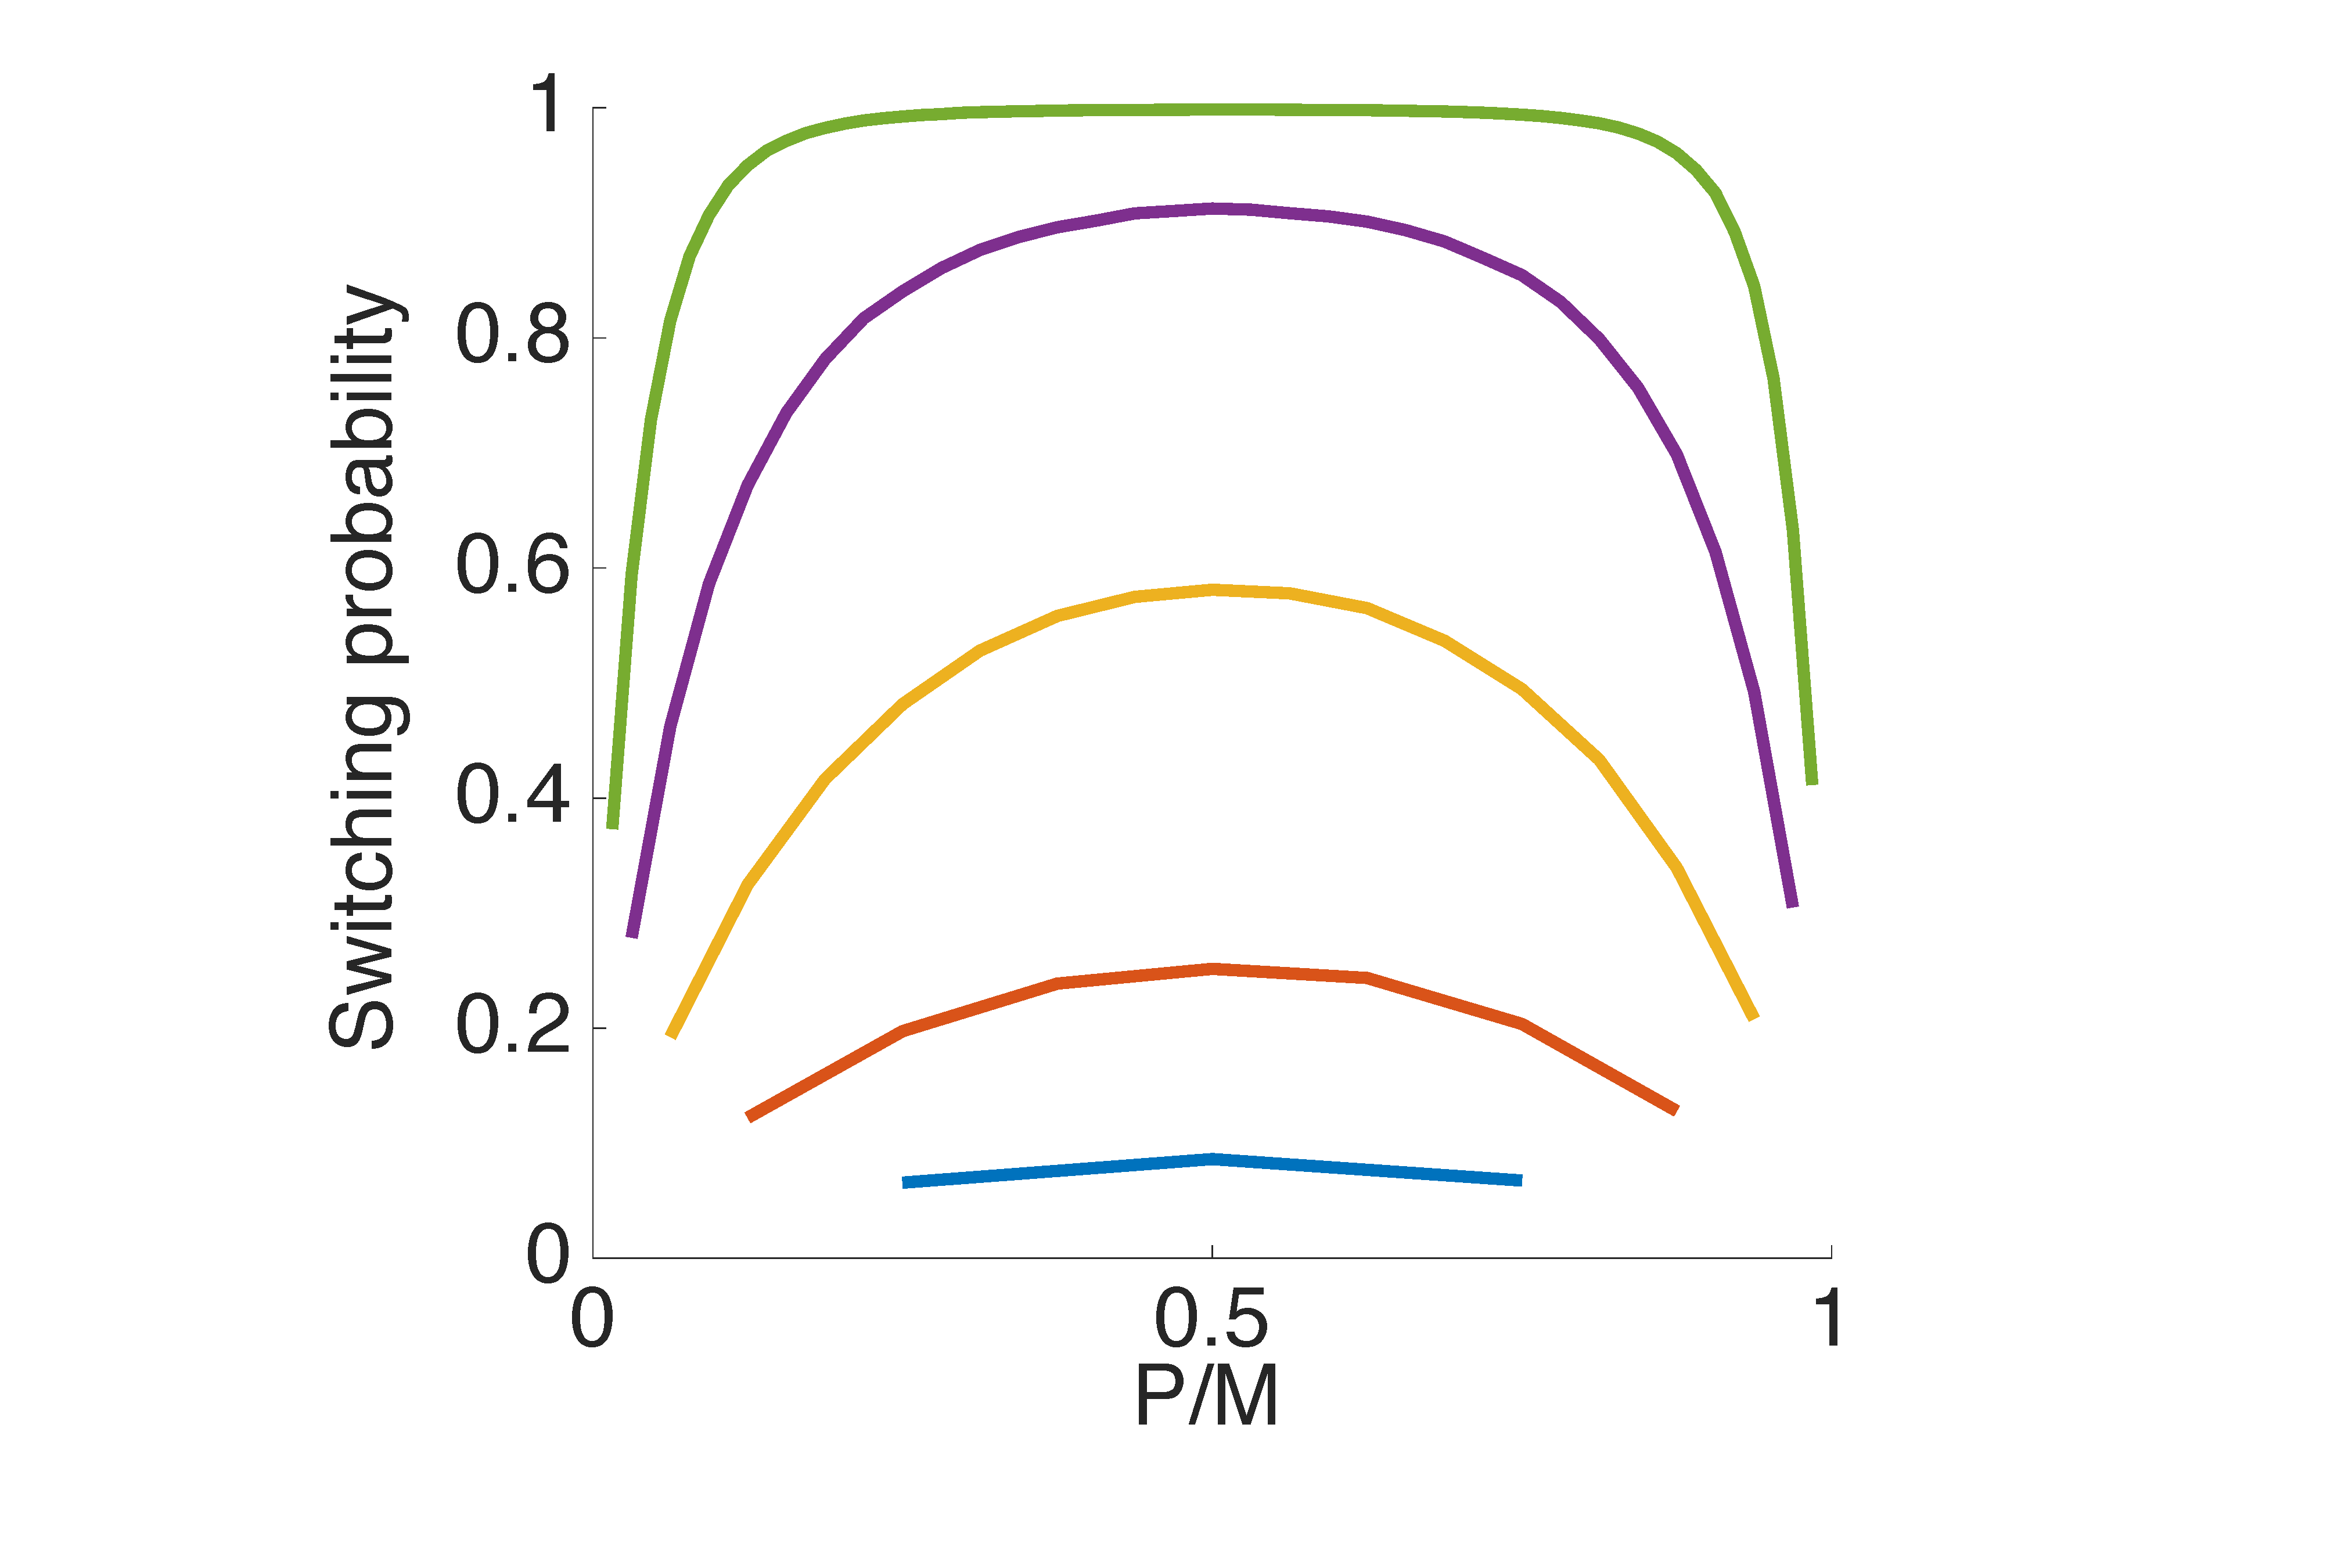
\includegraphics[height=0.75\textwidth]{swtiching_prob_sweep_sigma_3}
		\caption{Limiting log-Normal\label{fig:theSwitchingProb}}
	\end{subfigure}
	~~~~~~~~~~~
	\begin{subfigure}[t]{0.4\textwidth}
		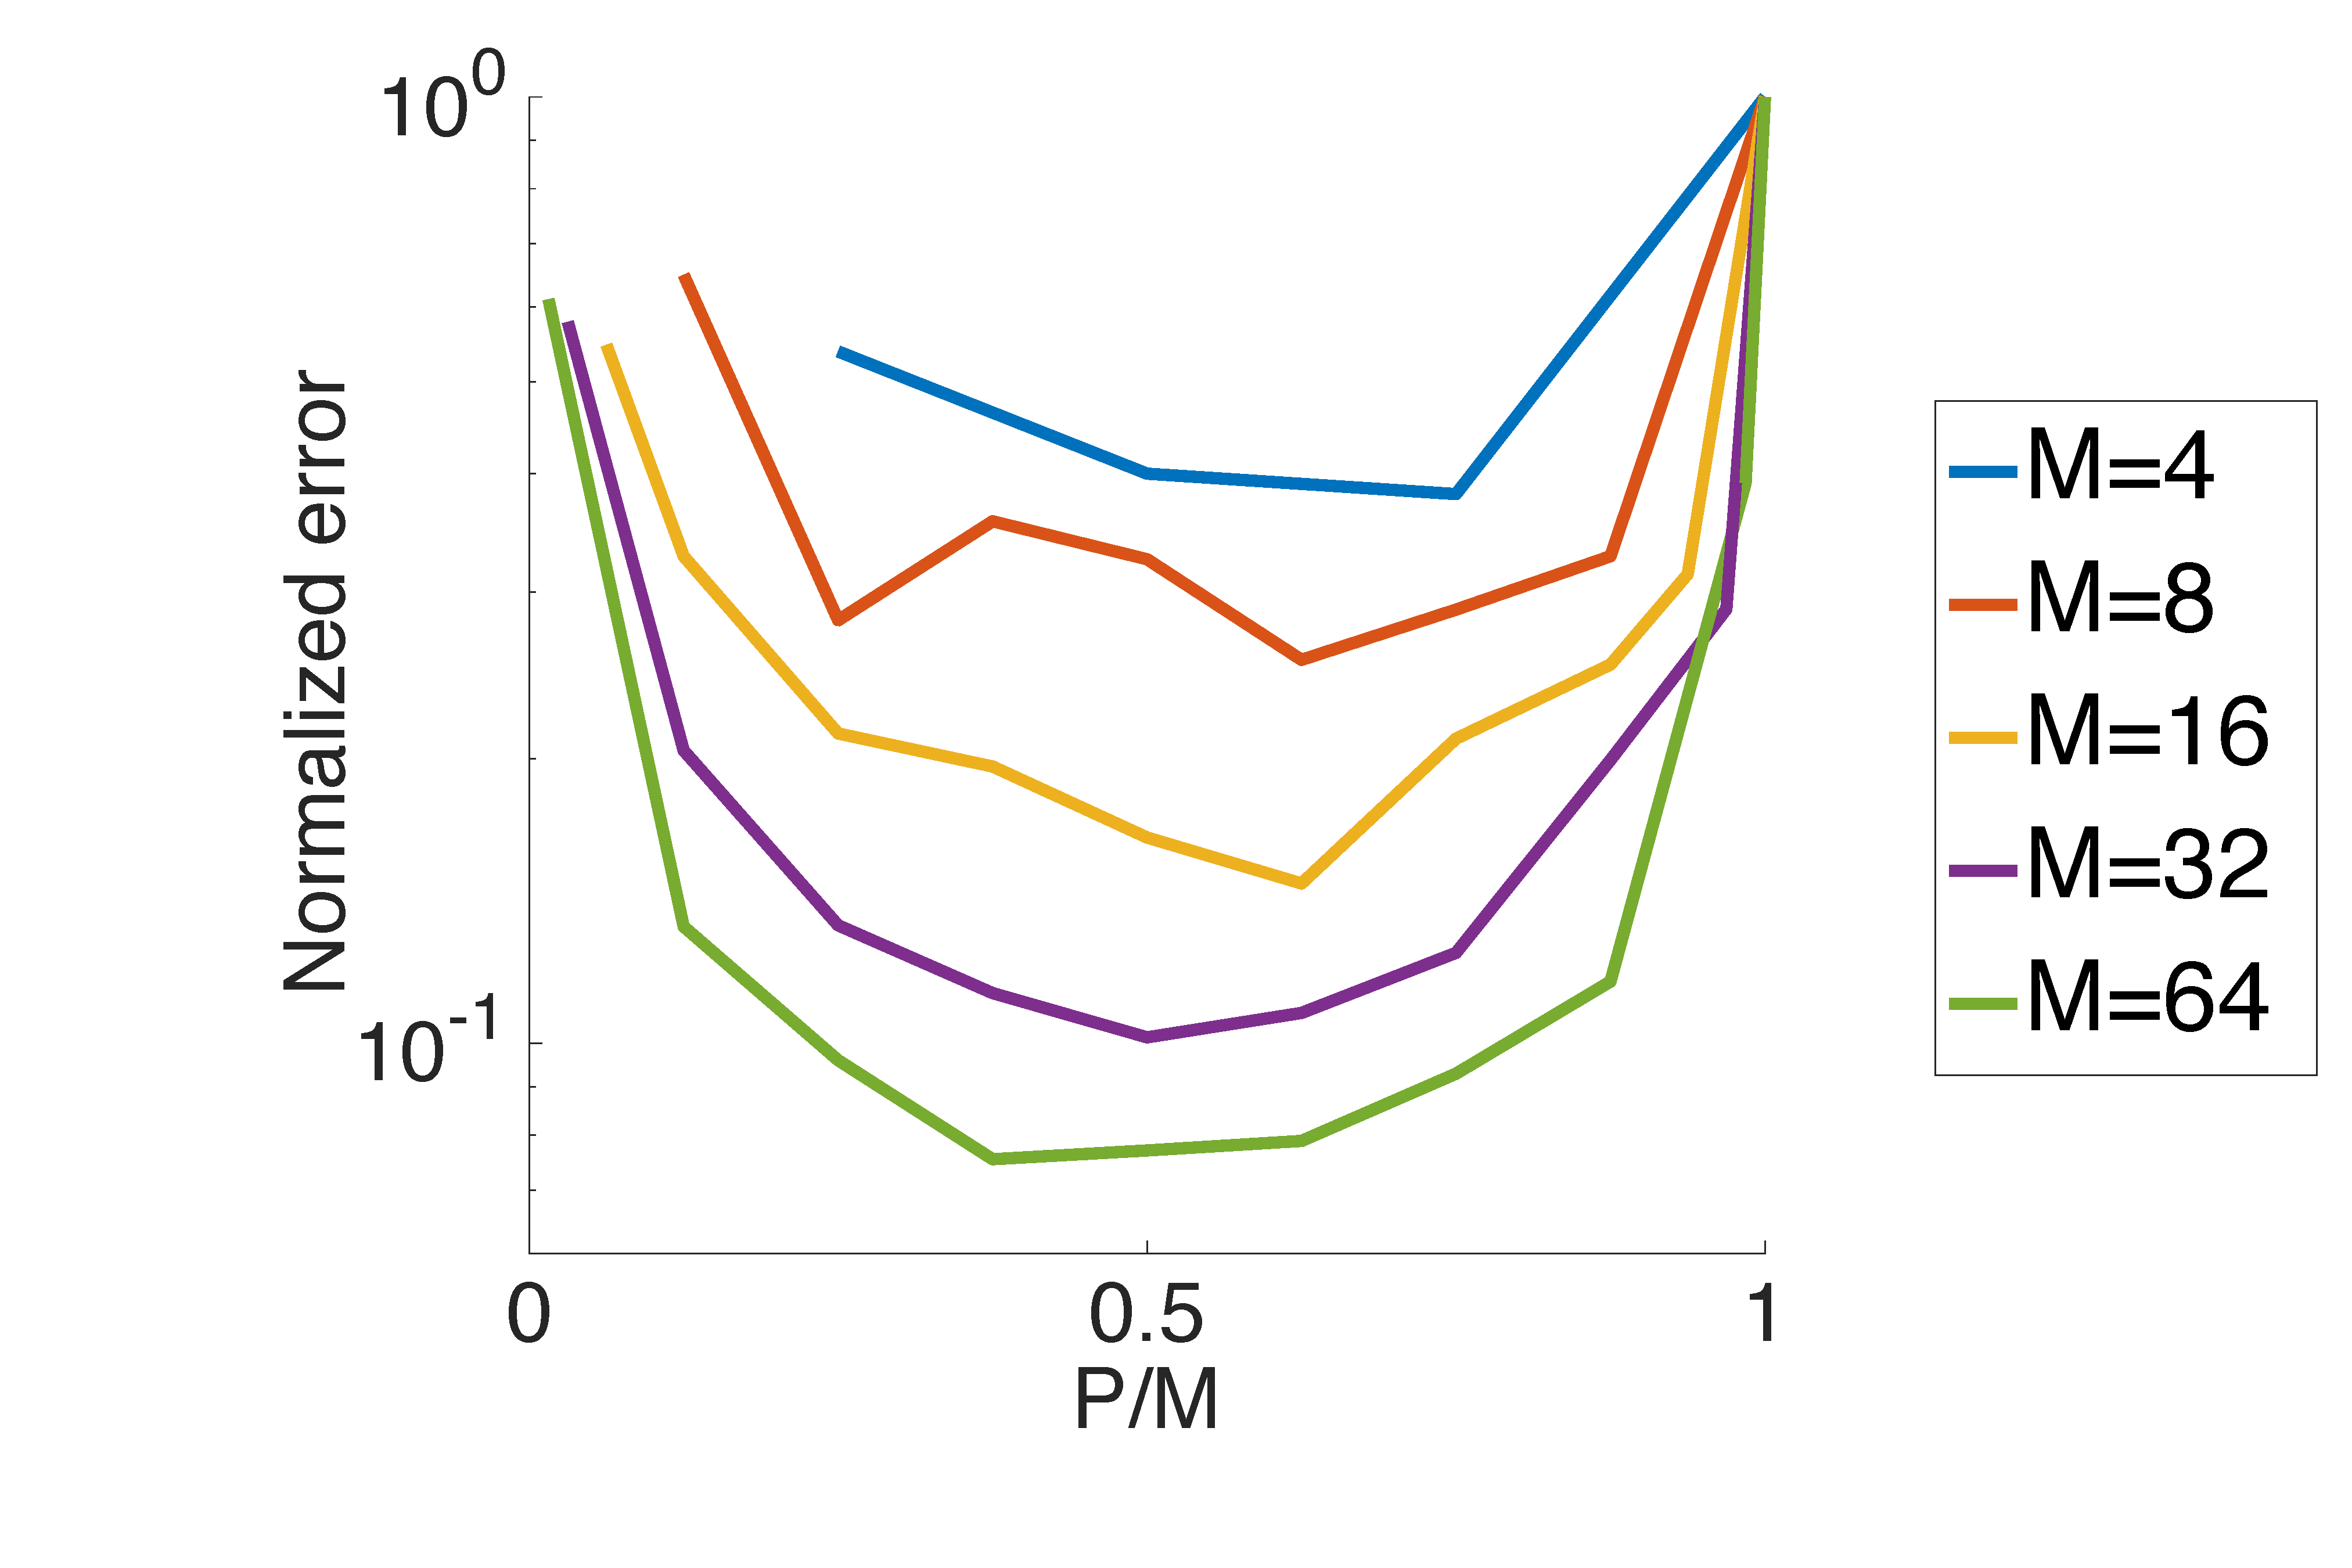
\includegraphics[height=0.75\textwidth]{big_font_p_sweep}
		\caption{Gaussian state space model\label{fig:Psweep}}
	\end{subfigure}
	\vspace{5pt}
	\caption{a) Estimation of switching probability for different choices of P and M assuming the log-Normal limiting distribution for $\hat{Z}_m$ with $\sigma=3$. b) Median error in mean estimate for different choices of P and M over 10 different synthetic datasets of the linear Gaussian state space model given in~\eqref{eq:LGSS} after 1000 MCMC iterations. Here errors are normalized by the error of a multi-start PG sampler which is a special case of iPMCMC for which $P=M$ (see Section \ref{sec:experiments}).
	}
\end{figure}

%
%\begin{figure}[h]
%
%\end{figure}
%~ %add desired spacing 

In practice we also see that best results are achieved when $P$ makes up roughly half of the nodes, see Figure~\ref{fig:Psweep} for performance on the state space model introduced in~\eqref{eq:LGSS}. Note also that the accuracy seems to be fairly robust with respect to the choice of $P$. % At least for this model, three things are clear from this sweep - firstly the optimal choice for the ratio of P/M is roughly 1/2, secondly that the performance of iPMCMC is relatively robust to changes in P around this optimum and thirdly that as $M$ increases, to relatively more preferable iPMCMC is to the trivial distribution of PG given by $P=M$ (this reason this occurs is discussed in more detail in Section \ref{sec:discussion}). 
%
Based on these results, we set the value of $P=M/2$ for the rest of our experiments.

% !TEX root = ../../main.tex

% Numerical experiments section
\subsection{Experiments}
\label{sec:experiments}

To demonstrate the %validity and
empirical performance of iPMCMC we report experiments on two state space models.  
Although both the models considered are Markovian, we emphasise that iPMCMC goes far beyond this and can be applied to arbitrary graphical models. 
%For exposition we will focus our comparison to the trivial distribution, whereby $M$ independent PMCMC samplers are run in parallel, of PG, particle independent Metropolis-Hastings (PIMH) \cite{andrieuDH2010} and the alternate move PG sampler (APG) \cite{holenstein2009particle}. 
We will focus our comparison on the trivially distributed alternatives, whereby $M$ independent PMCMC samplers are run in parallel--these are PG, particle independent Metropolis-Hastings (PIMH) \cite{andrieuDH2010} and the alternate move PG sampler (APG) \cite{holenstein2009particle}. Comparisons to other alternatives, including independent SMC, serialized implementations of PG and PIMH, and running a mixture of independent PG and PIMH samplers, are provided in Appendix \ref{sec:supp-additionalFigures}.  None outperformed the methods considered here, with the exception of running a serialized PG implementation with an increased number of particles, requiring significant additional memory ($O(MN)$ as opposed to $O(M+N)$).

In PIMH a new particle set is proposed at each \mcmc step using an independent \smc sweep, which is then either accepted or rejected using the standard Metropolis-Hastings acceptance ratio. % \cite{andrieuDH2010}. %\cite{hastings1970monte}. 
APG interleaves PG steps with PIMH steps
%, alternating between \csmc updates and a Metropolis-Hastings step with an independent \smc proposal,
in an attempt to overcome the issues caused by path degeneracy in PG.  We refer to the trivially distributed versions of these algorithms as multi-start PG, PIMH and APG respectively (mPG, mPIMH and mAPG). 
We use Rao-Blackwellization, as described in \ref{sec:allparticles}, to average over all the generated particles for all methods, weighting the independent Markov chains equally for mPG, mPIMH and mAPG. We note that mPG is a special case of iPMCMC for which $P=M$.  For simplicity, multinomial resampling was used in the experiments, with the prior transition distribution of the latent variables taken for the proposal.  $M=32$ nodes and $N=100$ particles were used unless otherwise stated.  Initialization of the retained particles for iPMCMC and mPG was done by using standard SMC sweeps.

\subsubsection{Linear Gaussian State Space Model}
\label{sec:LGSS}
We first consider a linear Gaussian state space model (LGSSM) with 3 dimensional latent states $x_{1:T}$, 20 dimensional observations $y_{1:T}$ and dynamics given by %\cn{It seems you use deterministic initial conditions for $x_0$, reformulate the model so you have a prior $\mu(x_1)$ instead? (also follows notation above)}
\begin{subequations}
	\label{eq:LGSS}
	\begin{align}
	x_1 & \sim \mathcal{N} \left(\mu, V\right) \label{eq:LGSSa}\\
	x_t & = \alpha x_{t-1} + \delta_{t-1} \quad & \delta_{t-1} \sim \mathcal{N} \left(0, \Omega\right) \label{eq:LGSSb}\\
	y_t & = \beta x_{t} + \varepsilon_{t} \quad & \varepsilon_{t} \sim \mathcal{N} \left(0, \Sigma\right).
	\label{eq:LGSSc}
	\end{align}
\end{subequations}
We set $\mu = [0, 1, 1]^T$, $V = 0.1 \; \mathbf{I}$, $\Omega = \mathbf{I}$ and $\Sigma = 0.1 \; \mathbf{I}$ where $\mathbf{I}$ represents the identity matrix.  The constant transition matrix, $\alpha$, corresponds to successively applying rotations of $\frac{7\pi}{10}$, $\frac{3\pi}{10}$ and $\frac{\pi}{20}$ about the first, second and third dimensions of $x_{t-1}$ respectively followed by a scaling of $0.99$ to ensure that the dynamics remain stable.  A total of 10 different synthetic datasets of length $T=50$ were generated by simulating from~\eqref{eq:LGSSa}--\eqref{eq:LGSSc}, each with a different emission matrix $\beta$ generated by sampling each column independently from a symmetric Dirichlet distribution with concentration parameter 0.2.

Figure \ref{fig:meanConv} shows convergence in the estimate of the latent variable means to the ground-truth solution for iPMCMC and the benchmark algorithms as a function of MCMC iterations.  It shows that iPMCMC comfortably outperforms the alternatives from around 200 iterations onwards, with only iPMCMC and mAPG demonstrating behaviour consistent with the Monte Carlo convergence rate, suggesting that mPG and mPIMH are still far from the ergodic regime.  Figure \ref{fig:meanPos} shows the same errors after $10^4$ MCMC iterations as a function of position in state sequence.  This demonstrates that iPMCMC outperformed all the other algorithms for the early stages of the state sequence, for which mPG performed particularly poorly. Toward the end of state sequence, iPMCMC, mPG and mAPG all gave similar performance, whilst that of mPIMH was significantly worse.


\begin{figure*}[t]
	\centering
	\begin{subfigure}[t]{0.49\textwidth}
		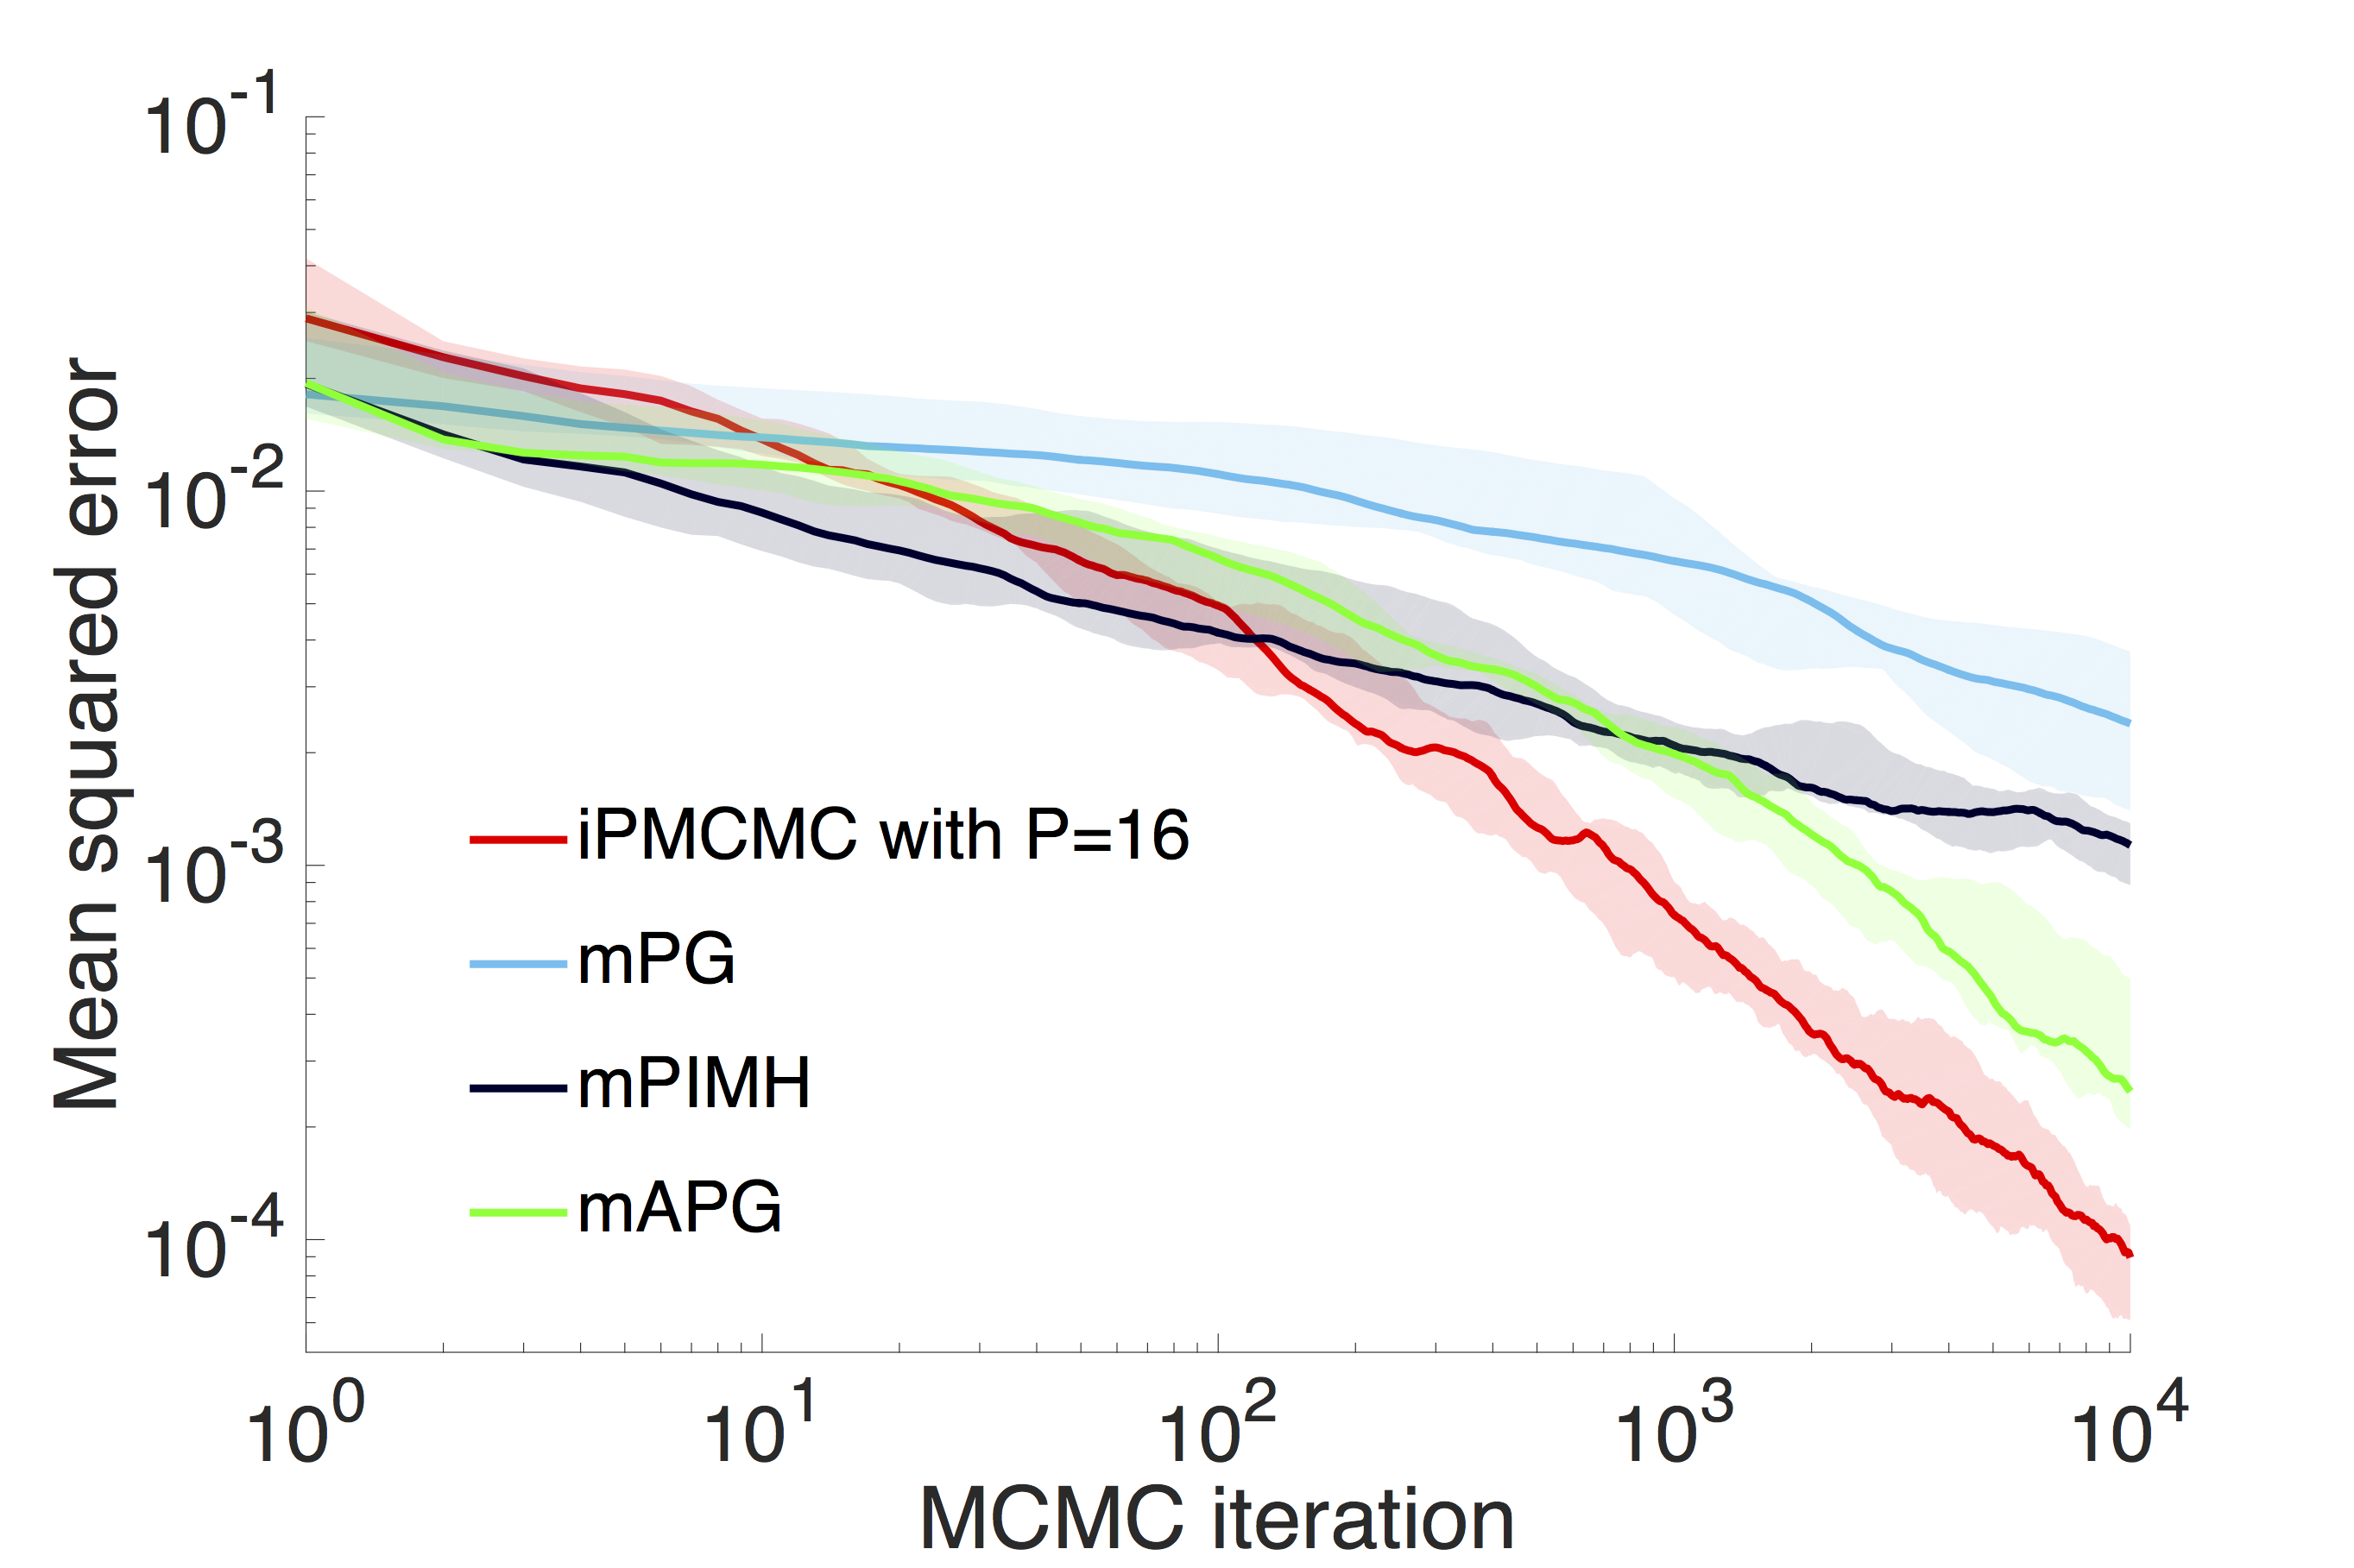
\includegraphics[width=\textwidth]{mean_conv_lss}
		\caption{Convergence in mean for full sequence}
		\label{fig:meanConv}
	\end{subfigure}
	~  %add desired spacing between images, e. g. ~, \quad, \qquad, \hfill etc. 
	%(or a blank line to force the subfigure onto a new line)
	\begin{subfigure}[t]{0.49\textwidth}
		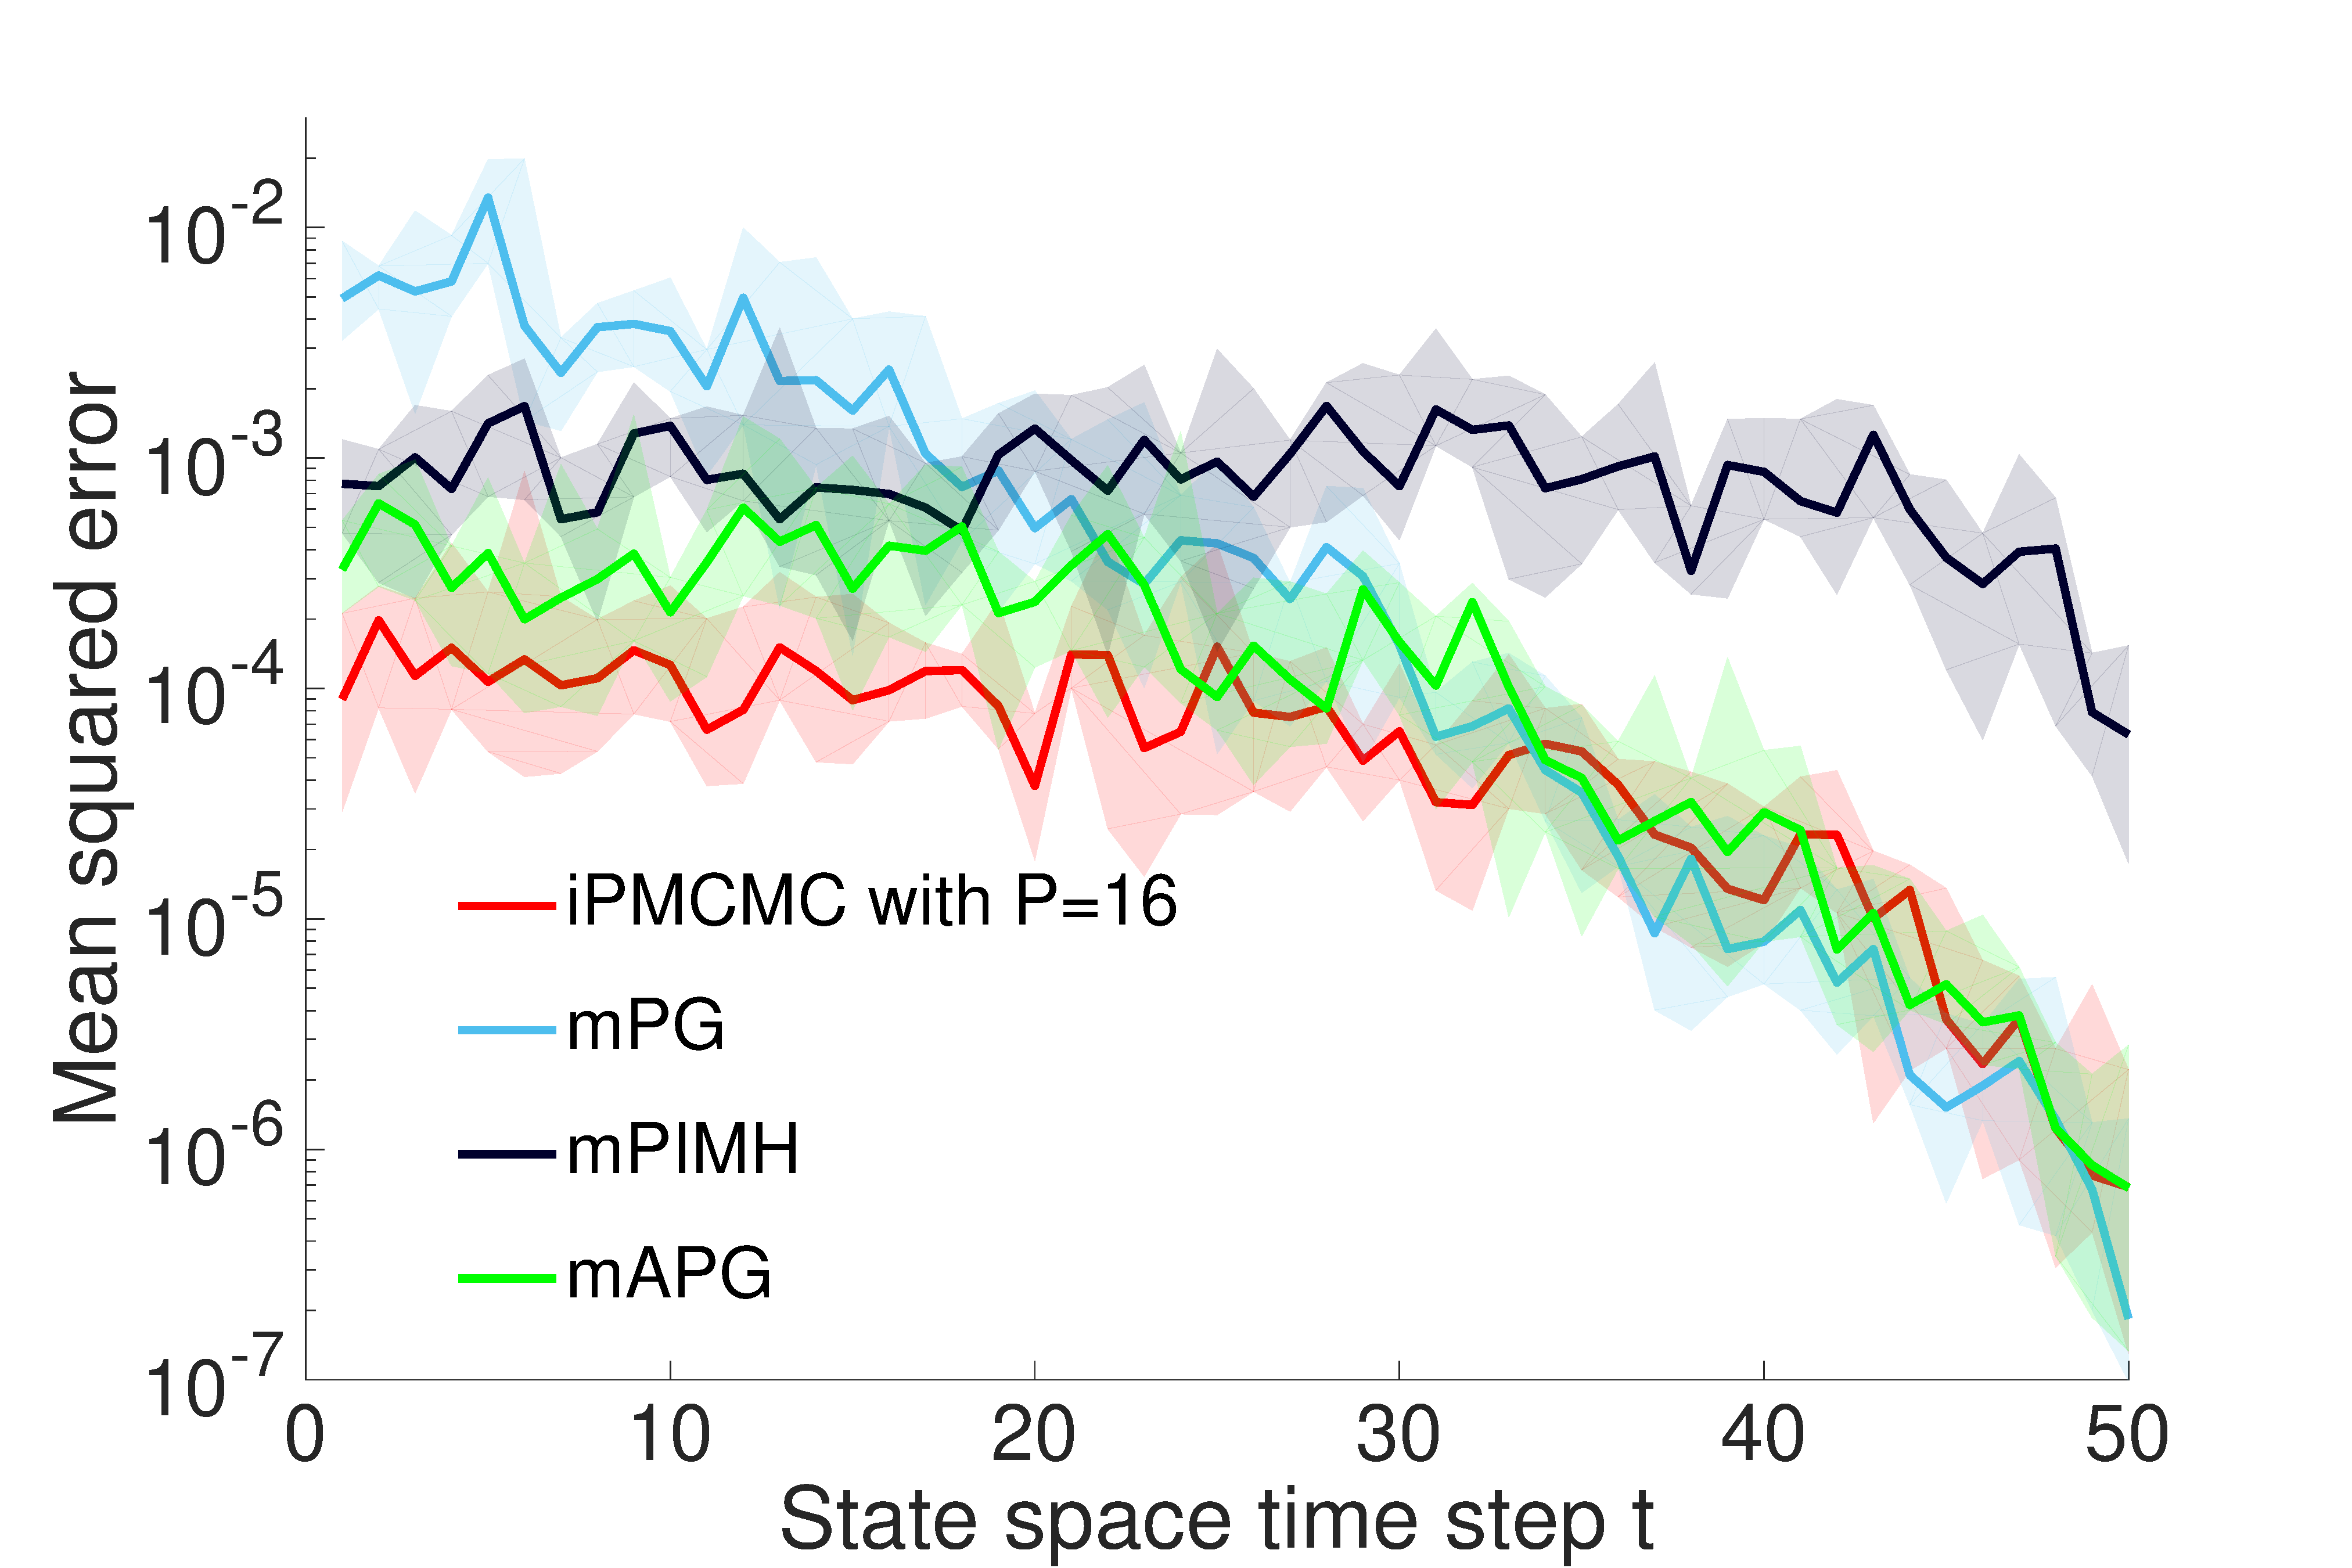
\includegraphics[width=\textwidth]{mean_pos_lss}
		\caption{Final error in mean for latent marginals}
		\label{fig:meanPos}
	\end{subfigure}
	
	%	\begin{subfigure}[t]{0.49\textwidth}
	%		\includegraphics[width=\textwidth]{std_conv_lss}
	%		\caption{Convergence in standard deviation for full sequence}
	%		\label{fig:stdConv}
	%	\end{subfigure}
	%	~ %add desired spacing between images, e. g. ~, \quad, \qquad, \hfill etc. 
	%	%(or a blank line to force the subfigure onto a new line)
	%	\begin{subfigure}[t]{0.49\textwidth}
	%		\includegraphics[width=\textwidth]{std_pos_lss}
	%		\caption{Final error in standard deviation for latent marginals}
	%		\label{fig:stdPos}
	%	\end{subfigure}	
	\caption{Mean squared error averaged over all dimensions and steps in the state sequence as a function of MCMC iterations (left) and mean squared error after $10^4$ iterations averaged over dimensions as function of position in the state sequence (right) for \eqref{eq:LGSS} with 50 time sequences.  The solid line shows the median error across the 10 tested synthetic datasets, while the shading shows the upper and lower quartiles.  Ground truth was calculated using the Rauch--Tung--Striebel smoother algorithm \cite{rauch1965maximum}. 
		\label{fig:groundTruth}}
\end{figure*}

\begin{figure*}[t]
	\centering
	\begin{subfigure}[t]{0.49\textwidth}
		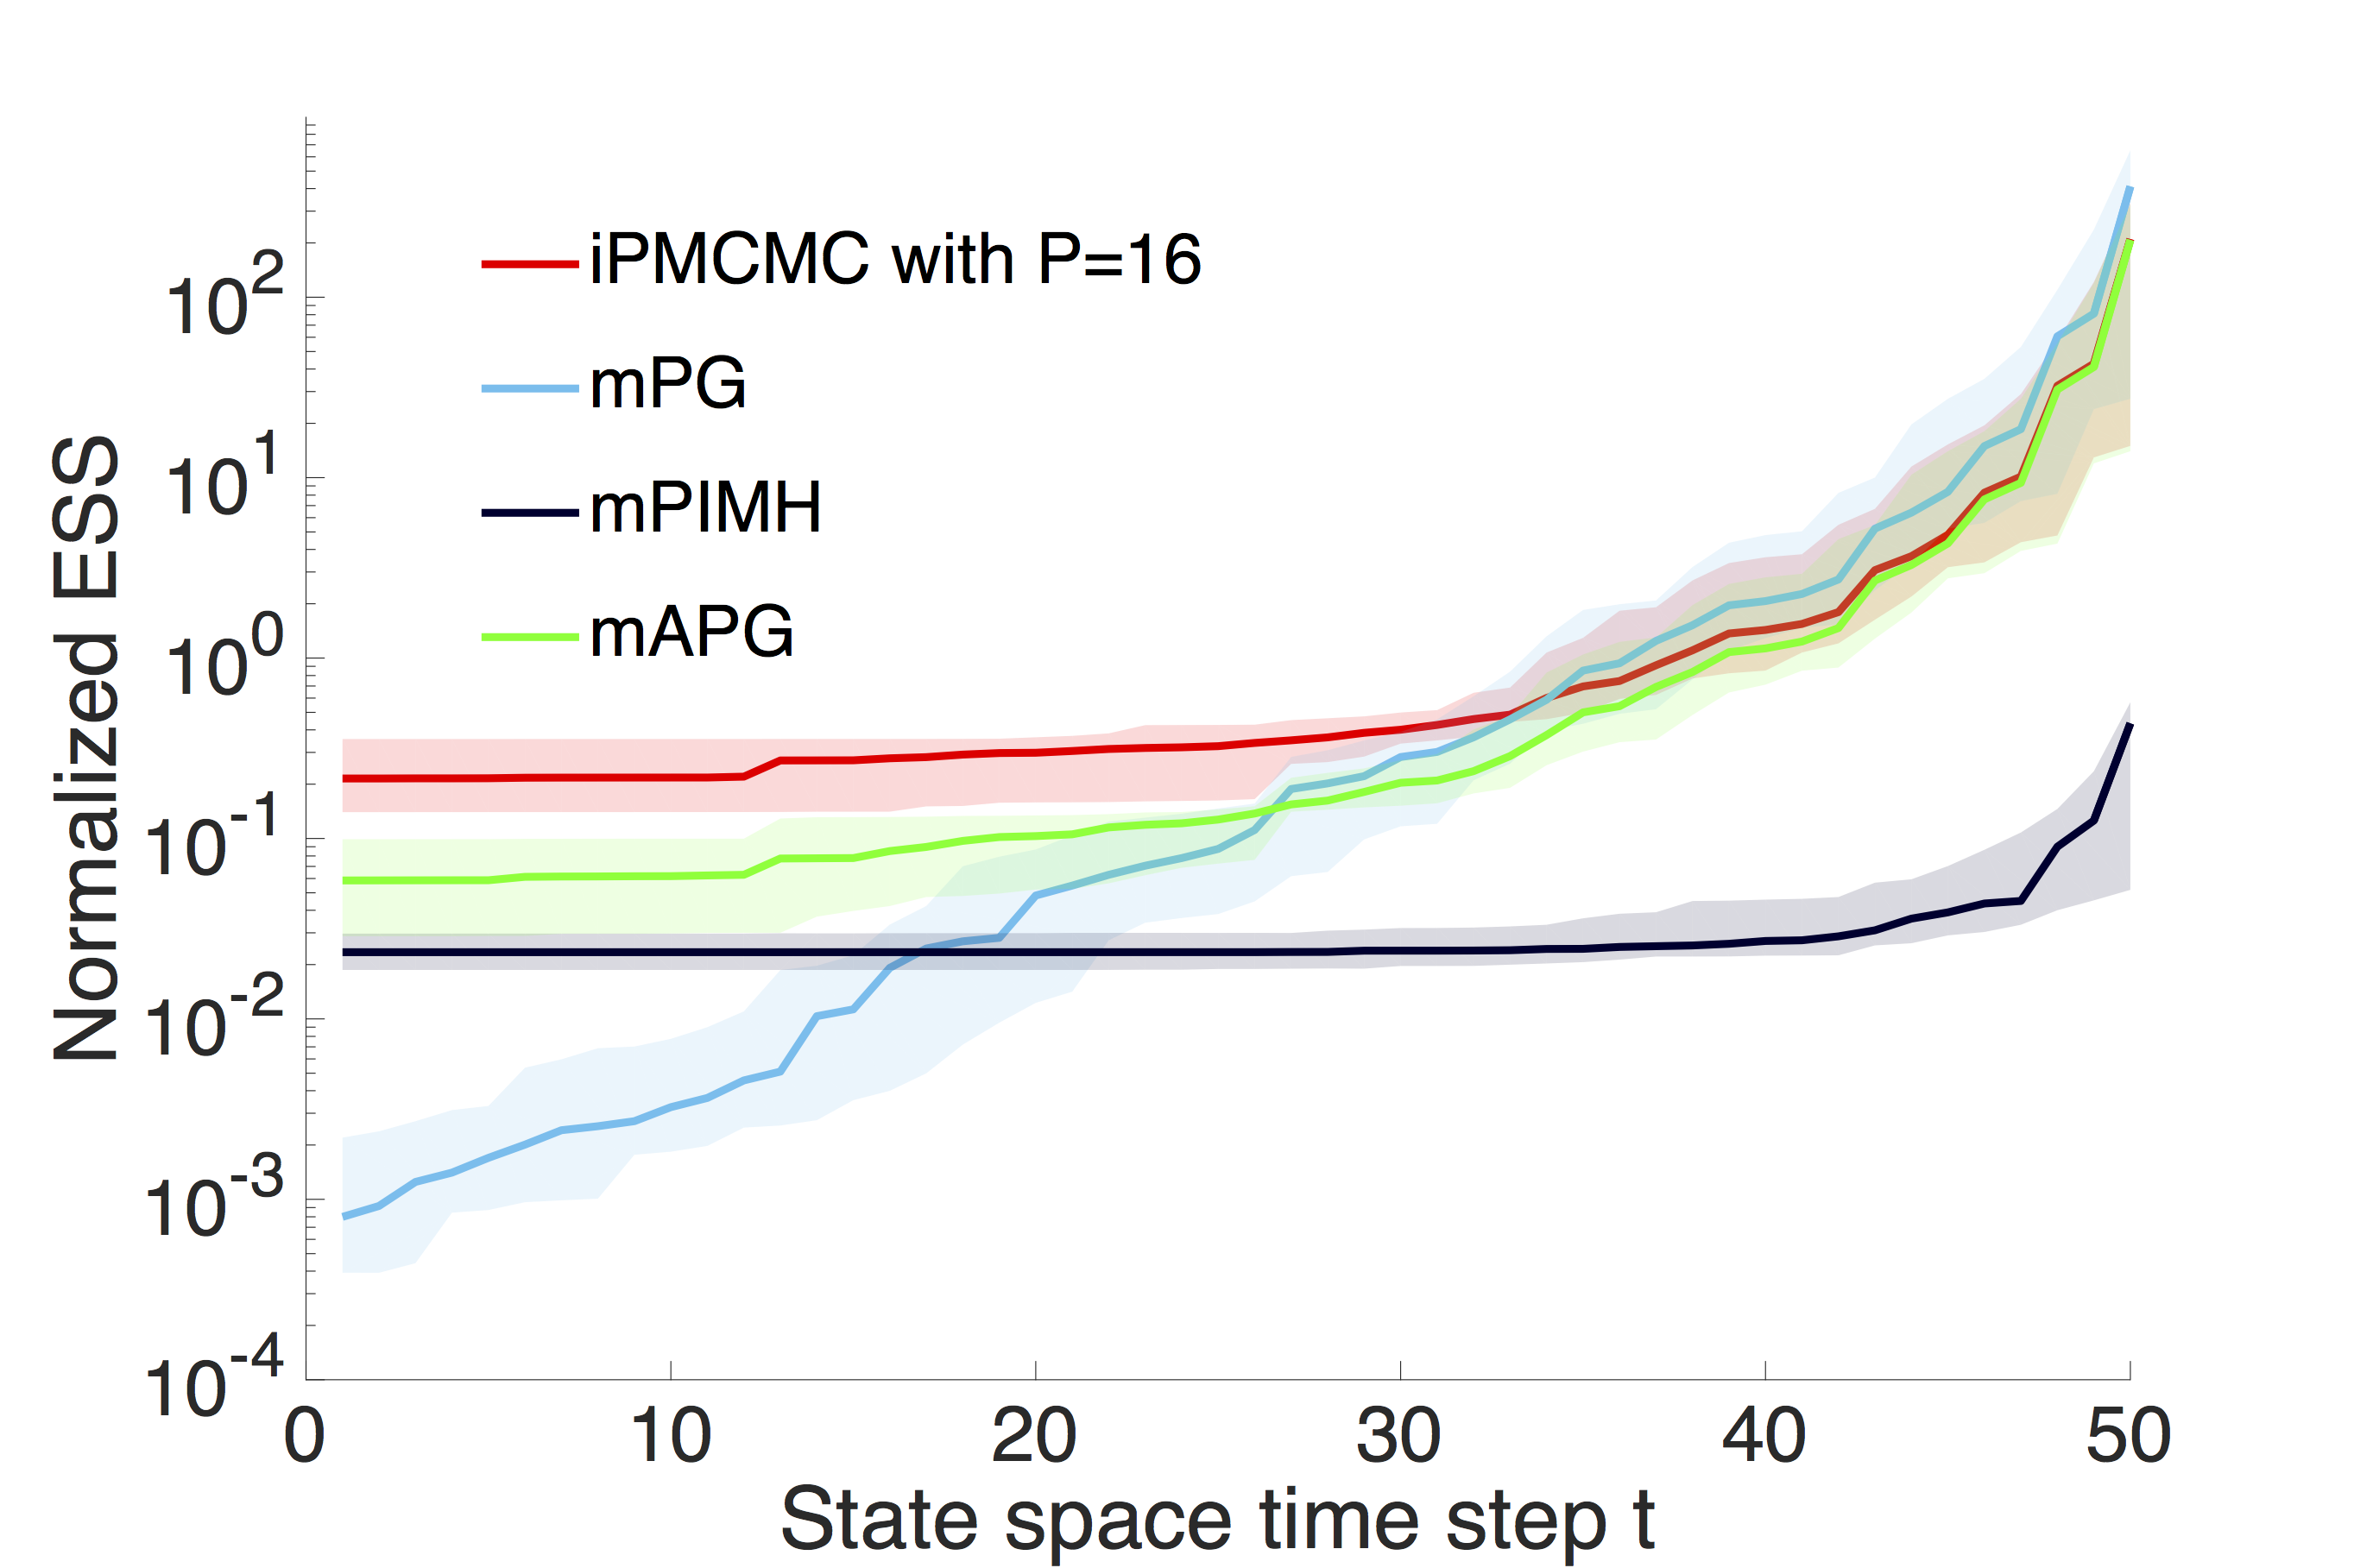
\includegraphics[width=\textwidth]{ess_lss}
		\caption{LGSSM}
	\end{subfigure}
	~ %add desired spacing between images, e. g. ~, \quad, \qquad, \hfill etc. 
	%(or a blank line to force the subfigure onto a new line)
	\begin{subfigure}[t]{0.49\textwidth}
		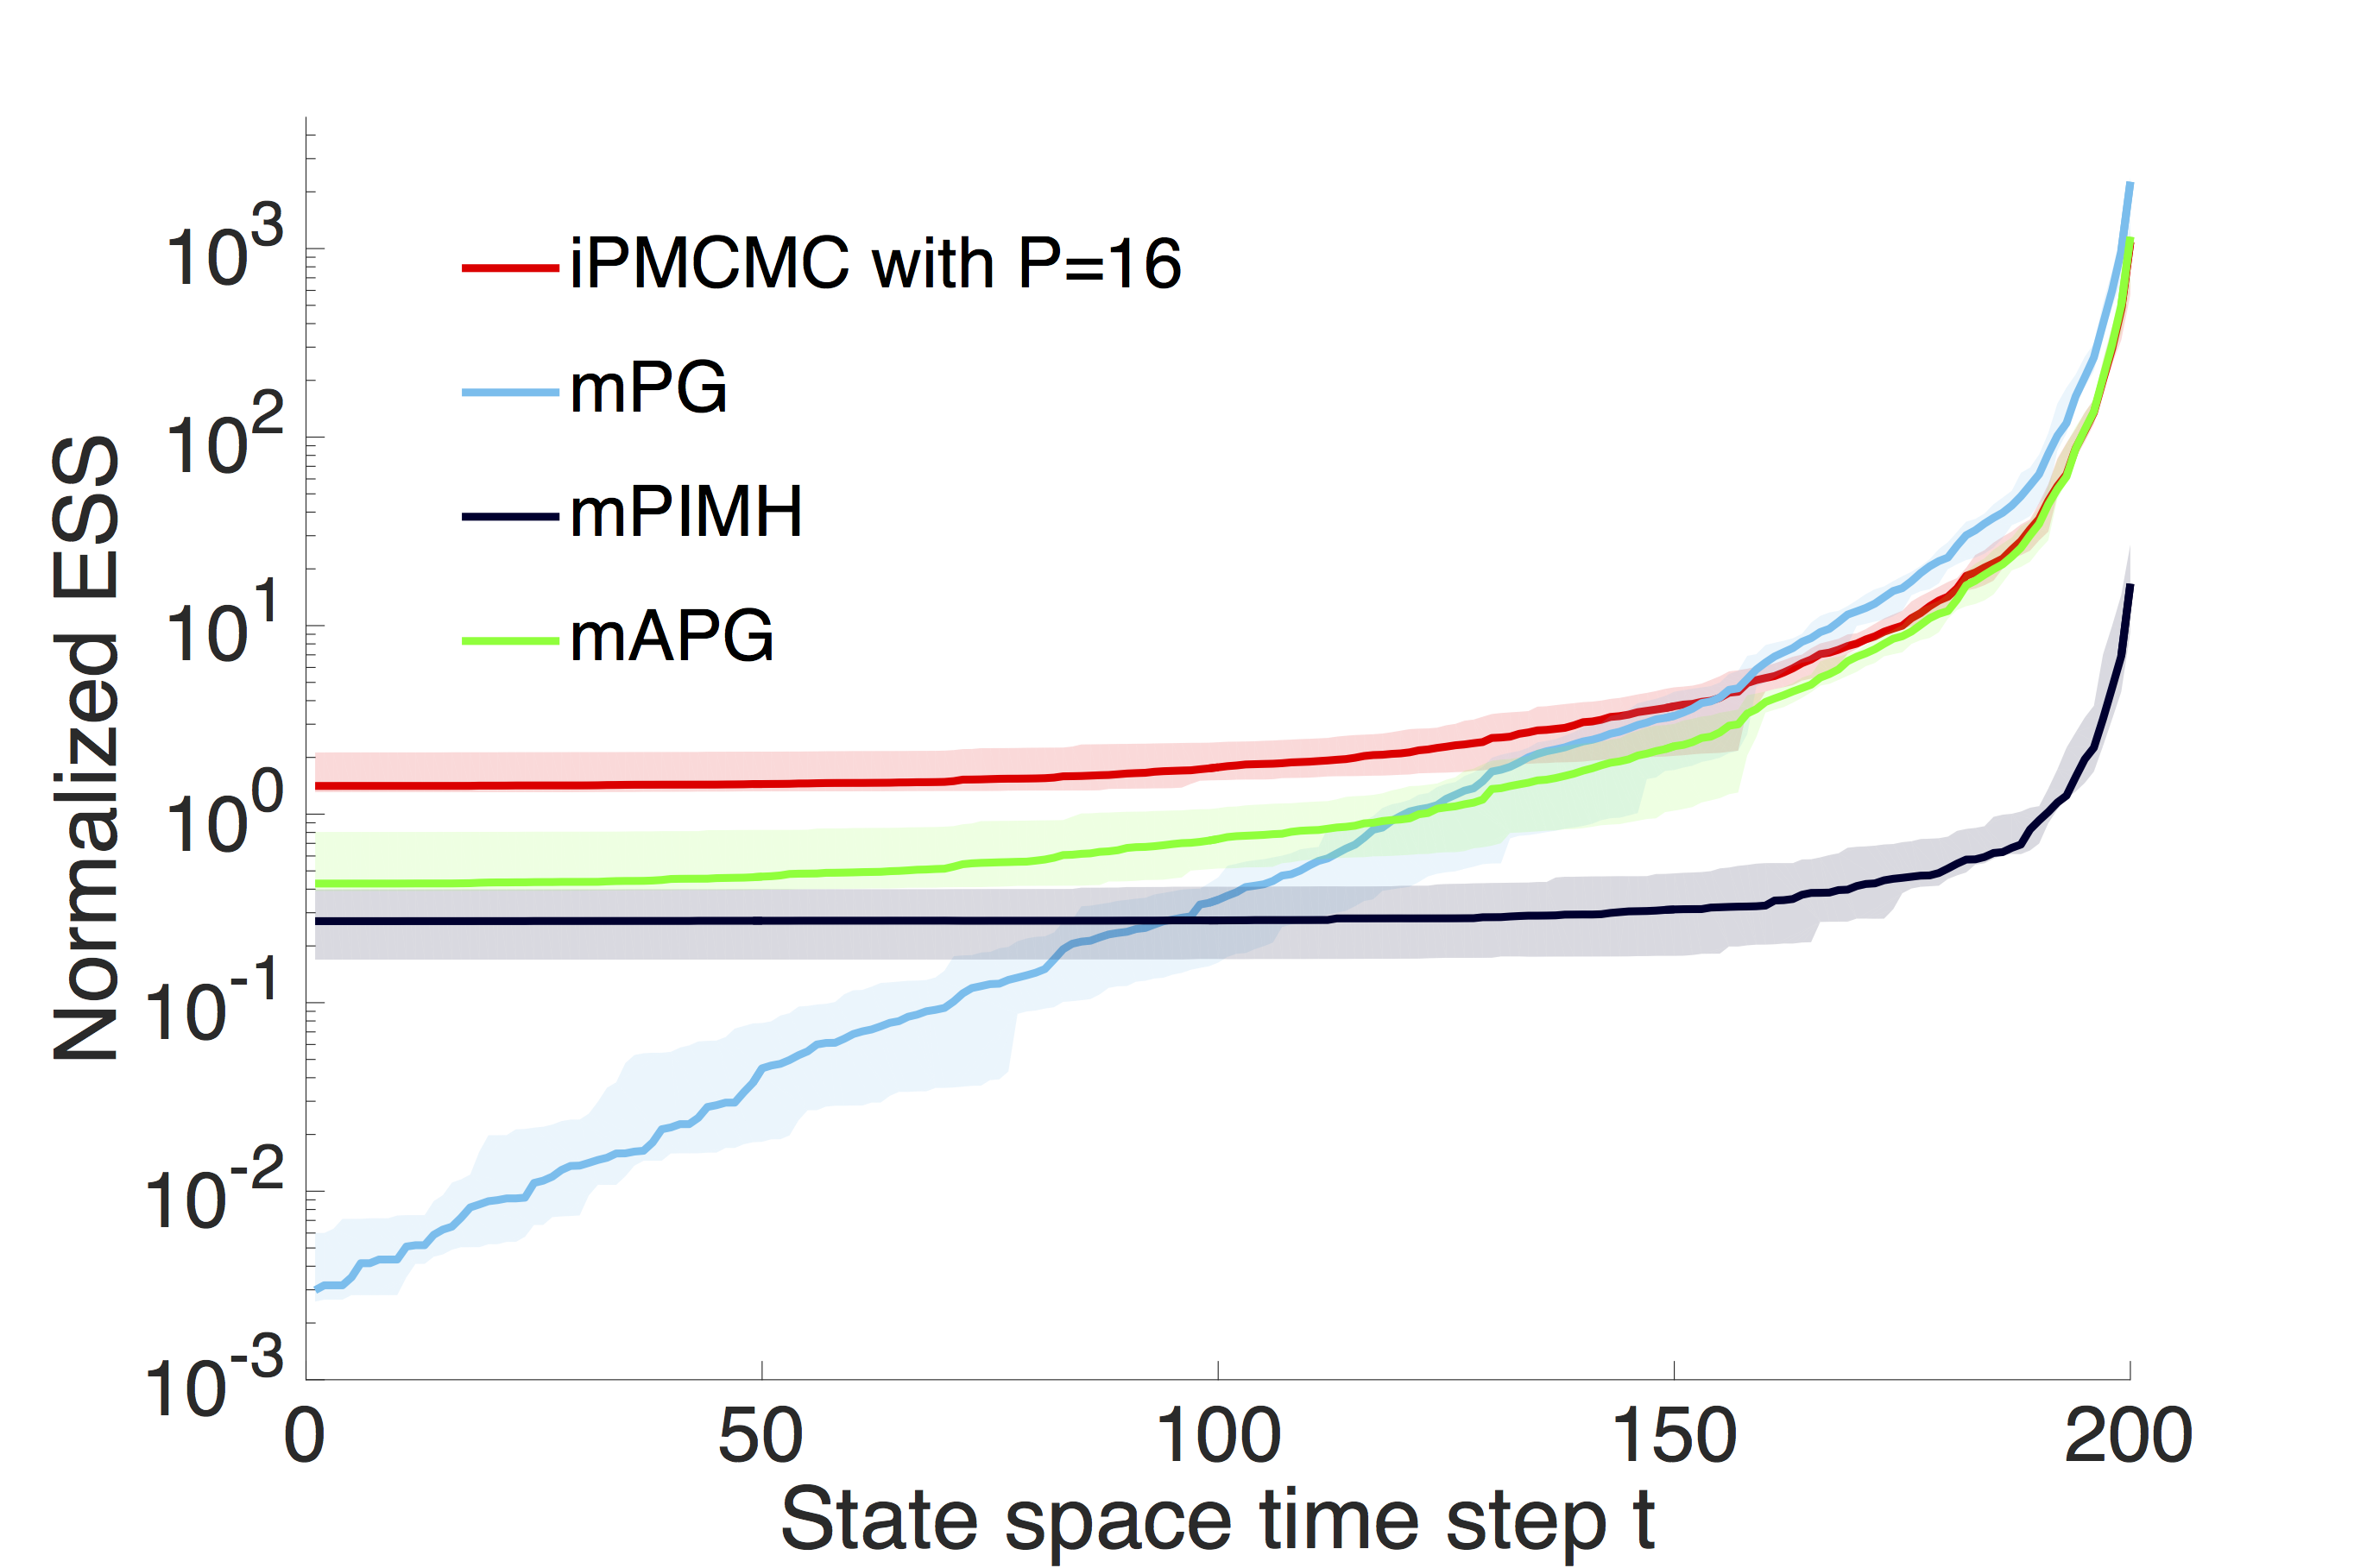
\includegraphics[width=\textwidth]{ess_nlss}
		\caption{NLSSM}
	\end{subfigure}
	
	\caption{Normalized effective sample size  (NESS) for LGSSM (left) and NLSSM (right).
		\label{fig:ESS}}
\end{figure*}

\subsubsection{Nonlinear State Space Model}
\label{sec:nlss}

We next consider the one dimensional nonlinear state space model (NLSSM) considered by, among others, \citet{gordon1993novel,andrieuDH2010}
\begin{subequations}
	\label{eq:NLSS}
	\begin{align}
	x_1 & \sim \mathcal{N} \left(\mu, v^2\right) \label{eq:NLSSa}\\
	x_t & = \frac{x_{t-1}}{2} + 25 \frac{x_{t-1}}{1+x_{t-1}^2} + 8 \cos \left(1.2t\right) + \delta_{t-1} \label{eq:NLSSb} \\
	y_t & = \frac{{x_{t}}^2}{20} + \varepsilon_{t} \label{eq:NLSSc}
	\end{align}
\end{subequations}
where $\delta_{t-1} \sim \mathcal{N} \left(0, \omega^2\right)$ and $\varepsilon_{t} \sim \mathcal{N} \left(0, \sigma^2\right)$.  We set the parameters as $\mu = 0$, $v=\sqrt{5}$, $\omega = \sqrt{10}$ and $\sigma = \sqrt{10}$.  Unlike the LGSSM, this model does not have an analytic solution and therefore one must resort to approximate inference methods. 
% such as sampling.
Further, the multi-modal nature of the latent space makes full posterior inference over $x_{1:T}$ challenging for long state sequences. 

\begin{figure*}[t]
	\centering
	%\begin{subfigure}[t]{0.99\textwidth}
	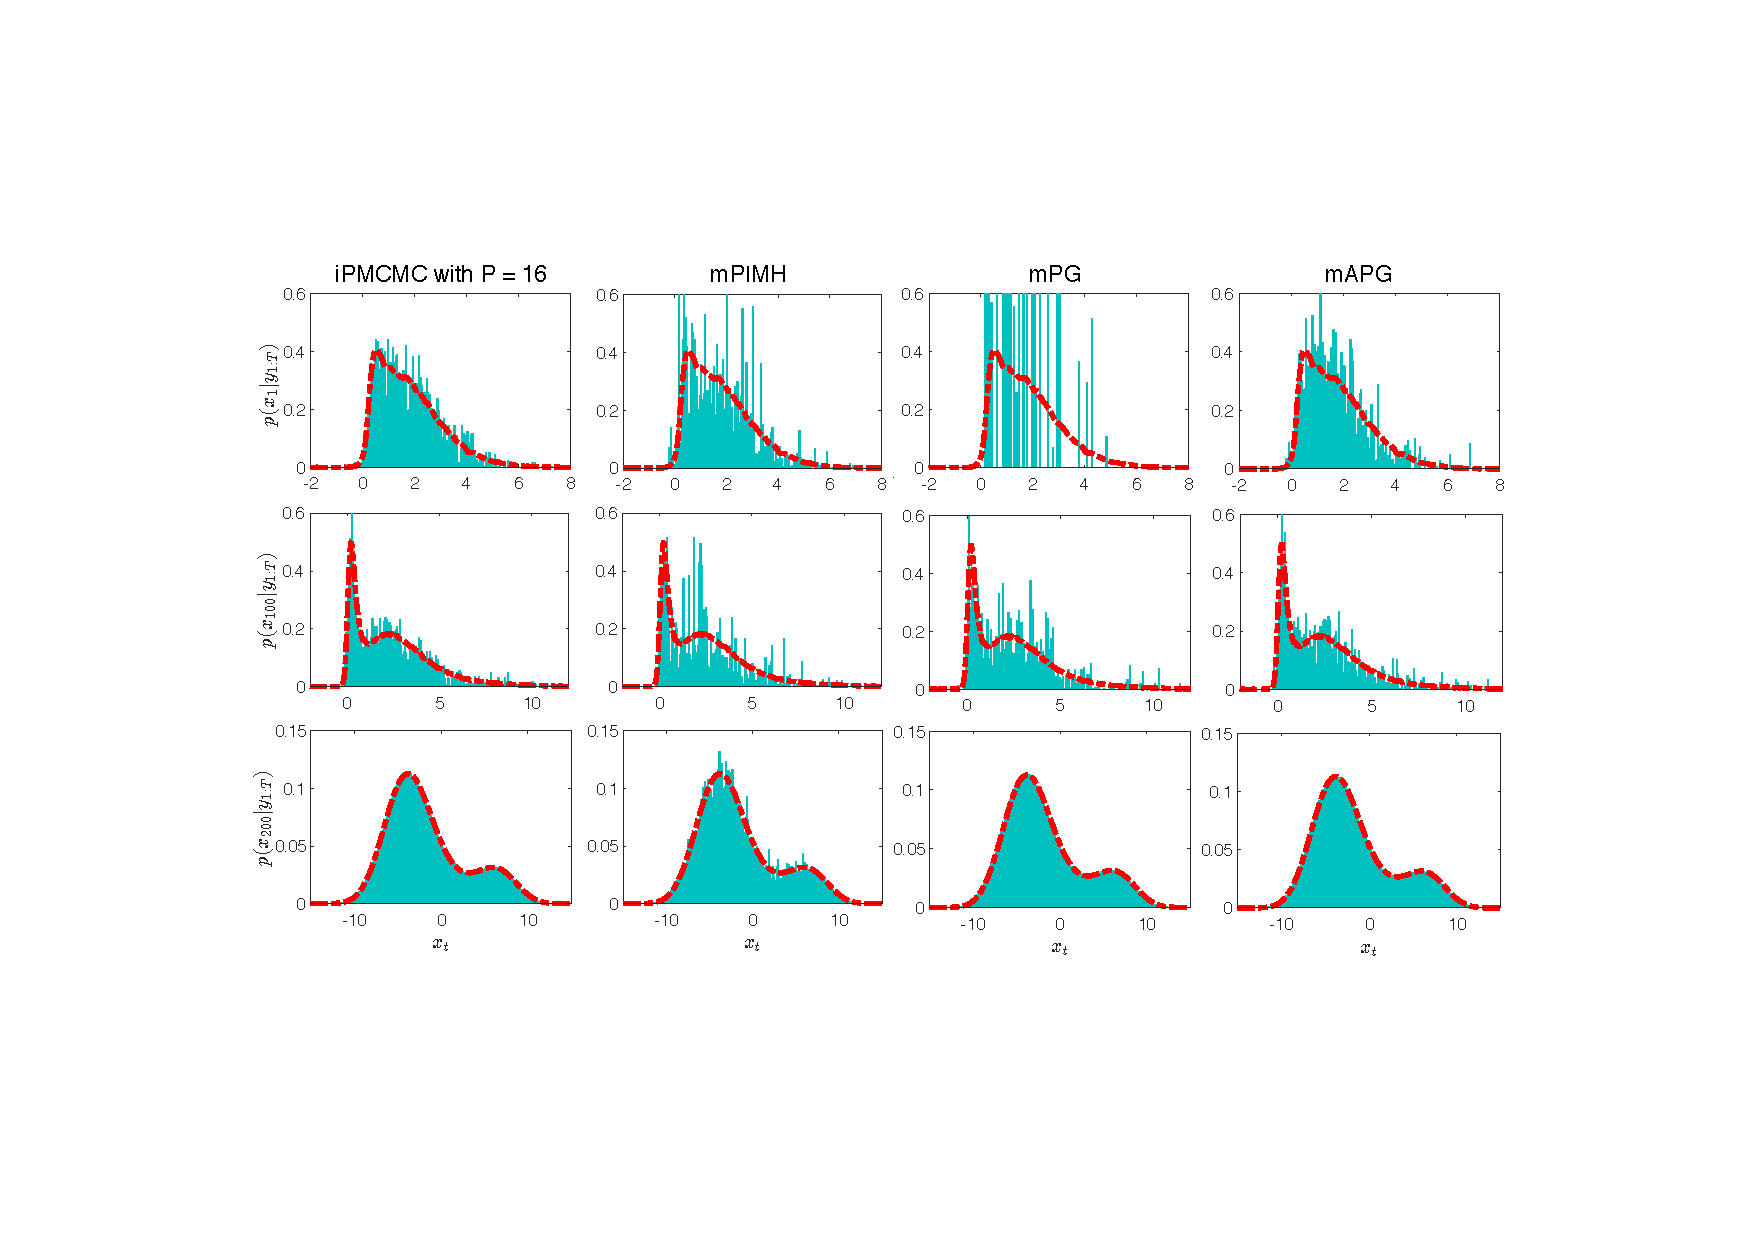
\includegraphics[width=1\textwidth]{nlss_histograms_minus_190.pdf}
	%\end{subfigure}
	\caption{Histograms of generated samples at $t=1, 100, \text{ and } 200$ for a single dataset generated from \eqref{eq:NLSS} with $T=200$.  Dashed red line shows an approximate estimate of the ground truth, found by running a kernel density estimator on the combined samples from a small number of independent SMC sweeps, each with $10^7$ particles. \label{fig:nlssHists}}
\end{figure*}

To examine the relative mixing of iPMCMC we calculate an effective sample size (ESS) for different steps in the state sequence.  In order to calculate the ESS, we condensed identical samples as done in for example \cite{vandemeent_aistats_2015}.  Let 
\begin{align*}
u_{t}^k \in \{x_{t,m}^{i}[r]\}^{i=1:N,r=1:R}_{m=1:M}, \quad \forall k \in 1 \dots K, \; t \in 1 \dots T
\end{align*} 
denote the unique samples of $x_t$ generated by all the nodes and sweeps of particular algorithm after $R$ iterations, where $K$ is the total number of unique samples generated.  The weight assigned to these unique samples, $v_t^{k}$, is given by the combined weights of all particles for which $x_t$ takes the value $u_{t}^k$:
\begin{align}
v_t^{k} = \sum_{r=1}^{R} \sum_{m=1}^{M} \sum_{i=1}^{N} \bar{w}_{t,m}^{i,r} \eta_{m}^{r} \delta_{x_{t,m}^{i}[r]}(u_{t}^{k})
\end{align}
where $\delta_{x_{t,m}^{i}[r]}(u_{t}^{k})$ is the Kronecker delta function and $\eta_{m}^{r}$ is a node weight.  For iPMCMC the node weight is given by as per the Rao-Blackwellized estimator described in Section~\ref{sec:allparticles}. For mPG and mPIMH, $\eta_{m}^{r}$ is simply $\frac{1}{RM}$,
as samples from the different nodes are weighted equally in the absence of interaction. 
Finally we define the effective sample size as $\text{ESS}_t = \left(\textstyle\sum_{k=1}^K \left(v_t^{k}\right)^2\right)^{-1}$.
%\begin{align}
%\label{eq:ESS}
%\text{ESS}_t = \left(\textstyle\sum_{k=1}^K \left(v_t^{k}\right)^2\right)^{-1}.
%\end{align}

Figure \ref{fig:ESS} shows the ESS for the LGSSM and NLSSM as a function of position in the state sequence.  For this, we omit the samples generated by the initialization step as this SMC sweep is common to all the tested algorithms.  We further normalize by the number of MCMC iterations so as to give an idea of the rate at which unique samples are generated.  These show that for both models the ESS of iPMCMC, mPG and mAPG is similar towards the end of the space sequence, but that iPMCMC outperforms all the other methods at the early stages. The ESS of mPG was particularly poor at early iterations.  PIMH performed poorly throughout, reflecting the very low observed acceptance ratio of around $7.3\%$ on average. 
%The lack of Monte Carlo convergence rate appearing in Figure \ref{fig:meanConv} also suggests this acceptance ratio is yet to converge, with the value in the ergodic regime likely to be even lower.   

It should be noted that the ESS is not a direct measure of performance for these models.  For example, the equal weighting of nodes is likely to make the ESS artificially high for mPG, mPIMH and mAPG, when compared with methods such as iPMCMC that assign a weighting to the nodes at each iteration.  To acknowledge this, we also plot histograms for the marginal distributions of a number of different position in the state sequence as shown in Figure \ref{fig:nlssHists}.  These confirm that iPMCMC and mPG have similar performance at the latter state sequence steps, whilst iPMCMC is superior at the earlier stages, with mPG producing almost no more new samples than those from the initialization sweep due to the degeneracy.  The performance of PIMH was consistently worse than iPMCMC throughout the state sequence, with even the final step exhibiting noticeable noise.

%An important feature of the ESS is that it is equal to the total number of samples ($NRM$) if all the samples are unique and have the same weight, and is equal to $1$ if there is only single unique sample with non-zero weight. It should be noted that ESS is not a direct measure of performance in the context of distributed PMCMC methods. In particular it takes no account of the suitability of the weights assigned to samples, for example the equal weighting assigned to different chains for mPG and mPIMH mean they will always have a higher ESS for a particle sweep \brooks{clarify ``particle sweep''?} than a iPMCMC sweep generating the same samples, regardless of whether this equal weighting gives a better approximation to the true posterior. \fredrik{I did not quite understand the last sentence.}

% !TEX root = ../../main.tex

% Discussion for things such as choice of P
\subsection{Discussion}
\label{sec:discussion}

The \ipmcmc sampler overcomes degeneracy issues in \pg by allowing the newly sampled particles from \smc nodes to replace the retained particles in \csmc nodes. Our experimental results demonstrate that, for the models considered, this switching in rate is far higher than the rate at which PG generates fully independent samples. Moreover, the results in Figure~\ref{fig:Psweep} suggest that the degree of improvement over an m\pg sampler with the same total number of nodes increases with the total number of nodes in the pool. 

The mAPG sampler performs an accept reject step that compares the marginal likelihood estimate of a single \csmc sweep to that of a single \smc sweep. In the \ipmcmc sampler the \csmc estimate of the marginal likelihood is compared to a population sample of \smc estimates, resulting in a higher probability that at least one of the \smc nodes will become a \csmc node.

%To explain the benefits of \ipmcmc  over mPIMH and mAPG methods consider a mAPG sampler where the PG and PIMH updates are out of sync for the different nodes such that at any particular MCMC iteration, half of the nodes are applying a PG update and the other half a PIMH update.  One could now informally view the sampling of the retained particles in mAPG as a simplified version of iPMCMC with $P=M/2$, except that the node-weights have been set equally and each of the unconditional SMC sweeps has been arbitrarily assigned as a proposal for one of the CSMC nodes.  Clearly this arbitrary assignment is detrimental as whilst the conditional nodes in iPMCMC consider both themselves and all the of the unconditional nodes for sampling a new retained particle, in mAPG they are restricted to drawing from either themselves or single alternative SMC sweep.  iPMCMC thus, in an informal sense, only requires the lowest of the CSMC node weights to be comparable to the highest of SMC node weights for switching to occur, whereas mAPG requires one of the arbitrary pairings to be comparable.  We therefore recommend setting $M$ as higher as possible, potentially even beyond the level of distribution available, noting the performance improvements of serialized PG shown in the supplementary material.



%Whenever PG degenerates to a single particle, this is guaranteed to correspond to the retained particle.  Therefore PG requires multiple particles to be retained from the start of the state sequence in order to generate new unique samples for all the latent variables in an MCMC iteration, causing it to become stuck at the same sample for variables early in the state sequence.  To quantify this improvement we note that $14.9\%$ of the retained particles produced by the iPMCMC sampler (after a short burn-in period), originated from unconditional SMC sweeps at the previous iteration.  Further, on average $85.4\%$ of the MCMC iterations for iPMCMC generated new retained particles for all stages of the state sequence. This contrasts with each PG sampler in mPG case producing an entirely new retained particle at a rate of only $0.076\%$.

%To explain the benefits of iPMCMC over mPIMH and mAPG consider a mAPG sampler where the PG and PIMH updates are out of sync for the different nodes such that at any particular MCMC iteration, half of the nodes are applying a PG update and the other half a PIMH update.  One could now informally view the sampling of the retained particles in mAPG as a simplified version of iPMCMC with $P=M/2$, except that the node-weights have been set equally and each of the unconditional SMC sweeps has been arbitrarily assigned as a proposal for one of the CSMC nodes.  Clearly this arbitrary assignment is detrimental as whilst the conditional nodes in iPMCMC consider both themselves and all the of the unconditional nodes for sampling a new retained particle, in mAPG they are restricted to drawing from either themselves or single alternative SMC sweep.  iPMCMC thus, in an informal sense, only requires the lowest of the CSMC node weights to be comparable to the highest of SMC node weights for switching to occur, whereas mAPG requires one of the arbitrary pairings to be comparable.  We therefore recommend setting $M$ as higher as possible, potentially even beyond the level of distribution available, noting the performance improvements of serialized PG shown in the supplementary material.

%Referring back to Figure~\ref{fig:Psweep}, we see that as $M$ is increased, the better the relative performance of iPMCMC.  As the reported errors are as a proportion of error given by mPG with the same $M$, this improvement is not simply because more computational resources have been allocated, but because the ``pool" from which the retained node indexes can be draw increases.  As the distribution in the ratio of CSMC node weights to SMC node weights is independent of $M$, the probability that all of the retained particles at the next MCMC iteration originate from the CSMC sweeps diminishes as shown by INSERT REF DEPENDING ON WHETHER IN SUP OR SEC XX.  The resulting improvement in performance with increasing $M$ seen in Figure~\ref{fig:Psweep} thus verifies the benefits from the increase interaction provided by iPMCMC.

Since the original \pmcmc paper in 2010 there have been several papers studying \citep{chopin2015,lindsten2015uniform} %\fredrik{Should we give some references to theoretical work on PG? for instance, I know of a paper in SJOS which is very good ;)}
and improving upon the basic \pg algorithm. Key contributions to combat the path degeneracy effect are backward simulation \citep{whiteley2010efficient,lindsten2013backward}
and ancestor sampling \citep{lindstenJS2014}. These can also be used to improve the \ipmcmc method ever further.  

%Noting that the Gibbs update in \eqref{eq:simConditional} requires no interaction between the \csmc nodes, iPMCMC should be amenable to an asynchronous adaptation under the assumption of a random execution time, independent of $\xb'$, in Algorithm~\ref{alg:csmc}.

%For this one would run a number of \smc nodes independently, communicating only their normalisation constant estimate and a sampled trajectory to a pool of possible retained particles with associated weights.  Whenever a \csmc sweep finishes its execution, it samples a new retained particle from either the pool or itself, replenishing the pool with a new sample if the new retained particle was not from the original \csmc sweep.  It should be noted that as this pool could be increased indefinitely, this adaptation has the potential to increase the scope and potential performance of iPMCMC even further.



% MOVED BACK TO METHODS
% Use backward sampling and/or ancestor sampling
%\subsection{Backward Simulation and Ancestor Sampling}
%Adding a backward or ancestor simulation step can drastically increase mixing when sampling the conditional trajectories $\xb_j'[r]$ \citep{lindsten2013backward}. In the \ipmcmc sampler we can replace simulating from the final weights on line~7 by a backward simulation step. Another option for the \csmc nodes is to replace this step by internal ancestor sampling \citep{lindstenJS2014} steps and simulate from the final weights as normal.

%
%\section{Other Methods and Extensions}
%
%\begin{itemize}
%	\item Backwards / ancestral sampling
%	\item Resample-move stuff
%	\item Rejuvenation
%\end{itemize}